\documentclass[10pt,a4paper,openright]{book}

\title{MATEMÁTICA DISCRETA Y LÓGICA}
\author{Juan Diego Barrado Daganzo\\1º de Carrera} %\\ es salto de linea
\date{\today}
\pagestyle{plain}
\setlength{\parskip}{0.35cm} %edicion de sangría
\setlength{\parindent}{0cm} %edicion de sangría
\clubpenalty=10000 %líneas viudas NO
\widowpenalty=10000 %líneas viudas NO

\usepackage[spanish]{babel} %Para que el idioma por defecto sea español
\usepackage{amsmath} %Paquetes para mates
\usepackage{amsfonts} %Paquetes para mates
\usepackage{amssymb} %Paquetes para mates
\usepackage{latexsym} %Paquetes para mates
\usepackage{cancel} %Paquete tachar cosas
\usepackage{multicol} %Paquetes columnas
\usepackage[top=2.5cm, bottom=2.5cm, left=3cm, right=3cm]{geometry}

\usepackage{titlesec} %Formato de capitulos y secciones
	\titleformat{\chapter}[display]{\normalfont\huge\bfseries\color{capitulos}}{\thechapter}{20pt}{\Huge}[\titlerule{}]
	\titleformat{\section}{\normalfont\Large\bfseries\color{secciones}}{\thesection}{1em}{}
	\titleformat{\subsection}{\normalfont\large\bfseries\color{subsecciones}}{\thesubsection}{1em}{}
	\titleformat{\subsubsection}{\normalfont\normalsize\bfseries\color{subsubsecciones}}{\thesubsubsection}{1em}{}

\usepackage[dvipsnames,usenames]{color} %activar e incluir colores
	\definecolor{capitulos}{RGB}{60,0,0}%gama de colores de los capitulos
	\definecolor{secciones}{RGB}{95,8,5}%gama de colores de las secciones
	\definecolor{subsecciones}{RGB}{140,36,31}%gama de colores de las subsections
	\definecolor{subsubsecciones}{RGB}{188,109,79}%gama de colores de las subsubsections

\usepackage{graphicx} %Para incluir fotos
\graphicspath{{./fotos/}}

\begin{document}
\maketitle

\mainmatter
\chapter*{LÓGICA ELEMENTAL}
\section*{PROPOSICIONES}
Las proposiciones son oraciones de sentido inequívoco que pueden ser ciertas o falsas. Usaremos habitualmente letras para referirnos a ellas: A, B, C, ...

\begin{itemize}
\item \textbf{Proposiciones compuestas}: solo pueden determinarse su veracidad por contraste con el mundo real
\item \textbf{Proposiciones atómicas}:formadas por las anteriores, su veracidad se puede determinar a partir de la combinación de las de las proposiciones atómicas que las componen.
\end{itemize}

\subsection*{\underline{Operaciones con proposiciones}}
\subsubsection*{Negación}
La proposición $A$ puede ser falsa o verdadera, pero $\neg A$ siempre será lo contrario de lo que sea $A$.
\begin{center}
 \begin{tabular}{|c|c|} 
   \hline
     $A$ & $\neg A$ \\ [0.5ex] 
   \hline \hline
     $V$ & $F$ \\
   \hline 
     $F$ & $V$ \\
   \hline
 \end{tabular}
\end{center}

\subsubsection*{Conjunción}
Es la ocurrencia de ambas proposiciones de forma simultánea, es decir, que ocurre tanto $P$ como $Q$.
\begin{center}
 \begin{tabular}{ |c|c|c| } 
   \hline
     $P$ & $Q$ & $P \wedge Q$ \\ [0.5ex] 
   \hline \hline
     $F$ & $F$ & $F$ \\
   \hline 
     $F$ & $V$ & $F$ \\
   \hline
     $V$ & $F$ & $F$ \\
   \hline
     $V$ & $V$ & $V$ \\
   \hline
 \end{tabular}
\end{center}

\subsubsection*{Disyunción}
Es la ocurrencia de una, otra o ambas proposiciones de forma simultánea, es decir, que ocurre o $P$, o $Q$ o tanto $P$ como $Q$.
\begin{center}
 \begin{tabular}{ |c|c|c| } 
   \hline
     $P$ & $Q$ & $P \vee Q$ \\ [0.5ex] 
   \hline \hline
     $F$ & $F$ & $F$ \\
   \hline 
     $F$ & $V$ & $V$ \\
   \hline
     $V$ & $F$ & $V$ \\
   \hline
     $V$ & $V$ & $V$ \\
   \hline
 \end{tabular}
\end{center}

\subsubsection*{Implicación}
Se suele expresar como si $P$, entonces $Q$ o $P$ implica $Q$. En este tipo de operaciones decimos que $P$ es la hipótesis o premisa y $Q$ la tesis o consecuencia\footnote{\scriptsize ¡¡¡Terminología importante!!! Decimos que P es condición suficiente para Q (basta que se cumpla P para concluir Q) y también, decimos que Q es condición necesaria para P puesto que para que $P \Rightarrow Q$ sea cierto, ha de cumplirse necesariamente Q cuando P es cierto (cuando $P \Rightarrow Q$ es cierto y Q es falso, también P debe ser falso).}. 

\begin{center}
 \begin{tabular}{ |c|c|c| } 
   \hline
     $P$ & $Q$ & $P \Rightarrow Q$ \\ [0.5ex] 
   \hline \hline
     $F$ & $F$ & $V$ \\
   \hline 
     $F$ & $V$ & $V$ \\
   \hline
     $V$ & $F$ & $F$ \\
   \hline
     $V$ & $V$ & $V$ \\
   \hline
 \end{tabular}
\end{center}

\subsubsection*{Recíproco de implicación}
Es la otra relación posible entre $A$ y $B$ y no es lo mismo puesto que las tablas de verdad son distintas.
\begin{center}
 \begin{tabular}{ |c|c|c| } 
   \hline
     $Q$ & $P$ & $Q \Rightarrow P$ \\ [0.5ex] 
   \hline \hline
     $F$ & $F$ & $V$ \\
   \hline 
     $F$ & $V$ & $V$ \\
   \hline
     $V$ & $F$ & $F$ \\
   \hline
     $V$ & $V$ & $V$ \\
   \hline
 \end{tabular}
\end{center}

\vspace{0.5cm}
Ej.: “Si un número es entero, entonces es racional”. Ser racional es una condición necesaria para poder ser entero.

\subsubsection*{Equivalencia}
“P es equivalente a Q” quiere decir que: $(P \Rightarrow Q) \wedge (Q \Rightarrow P)$. Se suele decir: “P si y solo si Q” o “P es necesario y suficiente”. De este modo, P y Q vienen a decir lo mismo o a expresar lo mismo.

\begin{center}
 \begin{tabular}{ |c|c|c|c|c| } 
   \hline
     $Q$ & $P$ & $P \Rightarrow Q$ & $Q \Rightarrow P$ & $P \Leftrightarrow Q$\\ [0.5ex] 
   \hline \hline
     $F$ & $F$ & $V$ & $V$ & $V$\\
   \hline 
     $F$ & $V$ & $F$ & $V$ & $F$\\
   \hline
     $V$ & $F$ & $V$ & $F$ & $F$\\
   \hline
     $V$ & $V$ & $V$ & $V$ & $V$\\
   \hline
 \end{tabular}
\end{center}

Ej.: “Un número es par si y solo si es divisible por 2”


\subsection*{\underline{Tautologías}}
Una tautología es una proposición o afirmación que es cierta para cualquier caso que se plantee. Para afianzar el concepto veamos unos ejemplos:
$$\neg(\neg A)\Leftrightarrow A$$
\begin{center}
 \begin{tabular}{ |c|c|c|c| } 
   \hline
     $A$ & $\neg A$ & $\neg (\neg A)$ & $\neg(\neg A)\Leftrightarrow A$ \\ [0.5ex] 
   \hline \hline
     $F$ & $V$ & $F$ & $V$ \\
   \hline 
     $V$ & $F$ & $V$ & $V$ \\
   \hline
 \end{tabular}
\end{center}

$$(A \Rightarrow B)\Leftrightarrow \neg (A \wedge \neg B)$$
\begin{center}
 \begin{tabular}{ |c|c|c|c|c|c| } 
   \hline
     $A$ & $B$ & $\neg B)$ & $\neg (A \wedge \neg B)$ & $A \Rightarrow B$ & $(A \Rightarrow B)\Leftrightarrow \neg (A \wedge \neg B)$ \\ [0.5ex]
      
   \hline \hline
     $F$ & $F$ & $V$ & $V$ & $V$ & $V$ \\
   \hline 
     $F$ & $V$ & $F$ & $V$ & $V$ & $V$\\
   \hline
     $V$ & $F$ & $V$ & $F$ & $F$ & $V$ \\
   \hline
     $V$ & $V$ & $F$ & $V$ & $V$ & $V$ \\
   \hline 
 \end{tabular}
\end{center}

\subsubsection*{Contraposición}
La contraposición es una tautología que establece una equivalencia entre una implicación ya dada y su contrapuesta:
$$(A \Rightarrow B) \Leftrightarrow (\neg B \Rightarrow \neg A)$$
$P:"x>3"$ \\
$Q:"x > 2"$ \\
$P \Rightarrow Q:"Si x>3, entonces x>2"$ \\
$\neg Q \Rightarrow \neg P:"Si x<2, entonces x<3"$ \\

\section*{LÓGICA DE PREDICADOS}
Con frecuencia nuestros enunciados y razonamientos cotidianos aluden a elementos o individuos de un colectivo, pero la Lógica Proposicional no recoge propiedades sobre individuos ni generalidades ni relaciones entre individuos para poder formalizarlos adecuadamente.\par
Por ejemplo:
\begin{itemize}
 \item “x es par”,
 \item “Algunos mamíferos leen”
 \item “Todos los que leen disfrutan”
\end{itemize}
Es necesario extender la Lógica Proposicional con nuevos elementos, dando lugar a un nuevo lenguaje formal más adecuado para las matemáticas, el lenguaje de la \textbf{Lógica de Primer Orden o Lógica de Predicados (LPO)}, se compone de:
\begin{itemize}
 \item \textbf{Dominio o universo de discurso}: colectivo de individuos sobre los que hablamos.
 \begin{center} Ej.: “x es par”, su dominio podría ser N \end{center}

 \item \textbf{Constantes}: nombres propios referidos a individuos.
	\begin{center} Ej.: 8, María, Juan.\end{center}

 \item \textbf{Variables}: Denotan valores cualesquiera del dominio. Representan individuos anónimos, generales.
	\begin{center} Ej.: x, y, …\end{center}

 \item \textbf{Predicados}: Enunciados sobre individuos. Pueden expresar propiedades de un individuo.
	\begin{center}Ej.: $P(x) \equiv x$ es par, $M(y) \equiv y$ es mamífero\end{center}

\indent También pueden expresar relaciones entre individuos.
	\begin{center}Ej.: $H(x,y) \equiv x$ e $y$ son hermanos \end{center} 

 \item \textbf {Funciones}: Descripción de un individuo en función de otro o de otros.
	\begin{center}  Ej.: $x+y,3·y,f(x)…$.\end{center}
\end{itemize}

\subsection*{\underline{Leyes de equivalencia}}
Dos proposiciones distintas $w_1$ y $w_2$ son equivalentes cuando sus valores de verdad son iguales en las mismas situaciones, es decir, las tablas de verdad son iguales.

\begin{multicols}{2}
\subsubsection*{Elemento neutro}
$$(w_1 \wedge V) \equiv w_1$$
$$(w_1 \vee F) \equiv w_1$$
\subsubsection*{Ley de absorción}
$$(w_1 \vee (w_1 \wedge w_2 )) \equiv w_1$$
$$(w_1 \wedge (w_1 \vee w_2 )) \equiv w_1$$
\subsubsection*{Ley de contradicción}
$$(w_1 \wedge \neg w_1 ) \equiv F$$
\subsubsection*{Ley del medio excluido}
$$(w_1 \vee \neg w_1) \equiv V$$
\subsubsection*{Leyes de dominación}
$$(w_1 \vee V) \equiv V$$
$$(w_1 \wedge F) \equiv F$$  
\subsubsection*{Ley de Idempotencia}
$$(w_1 \vee w_1) \equiv (w_1 \wedge w_1) \equiv V$$
\subsubsection*{Doble negación}
$$\neg \neg w_1 \equiv w_1$$
\subsubsection*{Leyes de De Morgan}
$$\neg (w_1 \vee w_2) \equiv \neg w_1 \wedge \neg w_2$$
$$\neg (w_1 \wedge w_2) \equiv \neg w_1 \vee \neg w_2$$  
\subsubsection*{Conmutatividad}
$$w_1 \vee w_2 \equiv w_2 \vee w_1$$
$$w_1 \wedge w_2 \equiv w_2 \wedge w_1$$
\subsubsection*{Leyes asociativas}
$$w_1 \vee w_2 \vee w_3 \equiv (w_1 \vee w_2) \vee w_3 \equiv w_1 \vee (w_2 \vee w_3)$$
$$w_1 \wedge w_2 \wedge w_3 \equiv (w_1 \wedge w_2 ) \wedge w_3 \equiv w_1 \wedge (w_2 \wedge w_3)$$  
\subsubsection*{Definición de condicional}
$$w_1 \Rightarrow w_2 \equiv \neg w_1 \vee w_2$$
\subsubsection*{Leyes distributivas}
$$w_1 \vee (w_2 \wedge w_3) \equiv (w_1 \vee w_2) \wedge (w_1 \vee w_3)$$
$$w_1 \wedge (w_2 \vee w_3) \equiv (w_1 \wedge w_2) \vee (w_1 \wedge w_3)$$
\subsubsection*{Contraposición}
$$w_1 \Rightarrow w_2 \equiv \neg w_2 \Rightarrow \neg w_1$$
\subsubsection*{Definición de equivalencia}
$$w_1 \Leftrightarrow w_2 \equiv (w_1 \Rightarrow w_2) \wedge (w_2 \Rightarrow w_1)$$
\end{multicols}

\subsection*{\underline{Cuantificadores}}
Los cuantificadores: \textit{existe}\footnote{Tras un existe se suele poner una CONJUNCIÓN.} y \textit{para todo}\footnote{Después de un \textit{para todo} SE DEBE ESCRIBIR UN PREDICADO (implicaciones, equivalencias…).}, se refieren a una propiedad relativa a un objeto $x$ o a todos los objetos de un cierto grupo.\par
Cuando queremos decir que existe un objeto $x$ que cumple una cierta propiedad o proposición, escribimos:
$$\exists x : P(x)$$
\scriptsize{(*)}\footnote{Los dos puntos:  significan \textit{Tal que}.}
\normalsize
$$\mbox{Ej.: } \exists x \in \mathbb R : (x>0) \wedge (\forall y \in \mathbb N : x \neq y)$$
Cuando queremos decir que todos los objetos de un cierto grupo tienen la propiedad $P(x)$:
$$\forall x : P(x)$$
$$\mbox{Ej.: }\forall x \in \mathbb R : x^2 \geq 0 \Rightarrow P(x)$$
Para referirse a que existe un ÚNICO $x$ que cumpla cierta proposición se utiliza el símbolo: $\exists !$, que se puede definir como: 
$$\exists !x : P(x)\Rightarrow \exists x : P(x) \wedge [\forall y : P(y) \Rightarrow y=x]$$
Para negar una proposición con cuantificadores, negamos todas sus partes:
$$\neg (\forall y : P(x))\Leftrightarrow \exists x : \neg P(x)$$
$$\neg (\exists x : P(x))\Leftrightarrow \forall x : \neg P(x)$$
Con varios cuantificadores y variables:
$$\neg (\forall x \exists y : P(x,y)) \Leftrightarrow \exists x \forall y : \neg P(x,y)$$
En general, los cuantificadores no conmutan:
$$\forall x \in D : (\exists y \in D : P(x))\neq \exists y \in D : (\forall x \in D : P(x,y))$$

\section*{MÉTODOS DE DEMOSTRACIÓN}
Una \textbf{demostración matemática} es una argumentación lógica que establece la verdad de una proposición matemática.\par
Un \textbf{sistema matemático} es tanto los hechos matemáticos de los que partes como los procesos de deducción que dan nuevos hechos matemáticos en un cierto campo de las matemáticas. Los sistemas matemáticos están formados por:
\vspace{0.5cm}
\begin{itemize}
\item \textbf{Axiomas}: proposiciones matemáticas siempre ciertas
\item \textbf{Definiciones}: permiten crear nuevos conceptos en base a los ya existentes
\item \textbf{Términos primitivos}: definidos mediante acuerdos o postulados
\item \textbf{Teoremas}: proposiciones matemáticas para las que se ha demostrado que son verdaderas
\item \textbf{Lemas}: teoremas pequeños para demostrar un teorema posterior
\item \textbf{Corolarios}: teoremas consecuencia de otros
\end{itemize}
La argumentación lógica es válida si la veracidad de las premisas de las que se parte conlleva necesariamente a la veracidad de la conclusión que se pretende demostrar, es decir, si no podemos concebir un escenario donde las premisas sean verdaderas y las conclusiones falsas.
\begin{equation*}
\begin{cases}
	\varphi_1 \\
	\varphi_2 \\
	... \\
	\varphi_n \\
\end{cases}
\vdash
\psi
\end{equation*}
Si una argumentación es válida, se dice que la conclusión se deduce lógicamente de las premisas, es decir, la proposición $\varphi_1 \wedge \varphi_2 \wedge ... \wedge \varphi_n \Rightarrow \psi$ debe ser verdadera y se denota como:
$$\{\varphi_1,\varphi_2, ...,\varphi_n\}\models \psi$$

\subsection*{\underline{Reglas de inferencia}}
Son las reglas empleadas en la argumentación, son válidas sencillas y permiten desarrollar la argumentación mediante su aplicación.
\begin{multicols}{2}
\subsubsection*{Modus Ponens}
$$\{A \Rightarrow B, A\}\vdash B$$
\subsubsection*{Modus Tollens}
$$\{A \Rightarrow B,\neg B\}\vdash \neg A $$
\subsubsection*{Silogismo Disyuntivo}
$$\{A \vee B, \neg B\}\vdash A$$
\subsubsection*{Conjunción}
$$\{A, B\}\vdash A\wedge B$$
\subsubsection*{Simplificación}
$$\{A\wedge B\}\vdash A$$
\subsubsection*{Demostración por casos}
$$\{A\Rightarrow C, B\Rightarrow C\}\vdash (A\vee B)\Rightarrow C$$
\subsubsection*{Adición}
$$\{A\}\vdash A\vee B$$
\subsubsection*{Silogismo Hipotético}
$$\{A\Rightarrow B, B\Rightarrow C\}\vdash A\Rightarrow C$$
\end{multicols}
\vspace{1cm}
Para las proposiciones con cuantificadores y en el ámbito del manejo de los mismos en la lógica:
\subsubsection*{Particularización universal}
$$\mbox{Si }\forall x \in D : P(x)\mbox{ es cierto, entonces }P(a) \mbox{ también es cierto siendo } a \mbox{ un elemento concreto de D}$$
\subsubsection*{Particularización existencial}
$$\mbox{Si }\exists x \in D : P(x)\mbox{ es cierto, entonces es cierto que }\exists a \in D : P(a)\mbox{ siendo } a \mbox{ un elemento concreto}$$
\subsubsection*{Generalización universal}
$$\mbox{Si }P(x)\mbox{ se satisface para un } x \mbox{ arbitrario, entonces } \forall x \in D : P(x)$$
\subsubsection*{Generalización existencial}
$$\mbox{Si }P(x)\mbox{ se satisface para un } x \mbox{ concreto de D, entonces } \exists x \in D : P(x)$$
\vspace{0.5cm}
\subsection*{\underline{Demostración directa}}
Basada en la tautología Modus ponens:
\begin{equation*}
[P\wedge (P\Rightarrow Q)]\Rightarrow Q
\end{equation*}
Lo que se puede traducir en:
\begin{equation*}
[P\wedge (P\Rightarrow R)]\wedge (R\Rightarrow T) \wedge ... \wedge (... \Rightarrow Q)]\Rightarrow Q
\end{equation*}

Ej.: “El cociente de números racionales es racional”
\begin{equation*}
a,b \in \mathbb Q \Rightarrow a=\frac{m}{n},b=\frac{k}{l}:m,n,k,l\in \mathbb Z \wedge n,l \neq 0
\end{equation*}
\begin{equation*}
\frac{a}{b}= \frac{\frac{m}{n}}{\frac{k}{l}}=\frac{ml}{nk}\Rightarrow ml,nk \in \mathbb Z \wedge b \neq 0 \Rightarrow k\neq 0 \Rightarrow n·k\neq 0 \Rightarrow \frac{a}{b} \in \mathbb Q
\end{equation*}

Ej.: “La suma de los cuadrados de dos números impares (enteros) es un número par”
\begin{eqnarray*}
m &=& 2k-1, k \in \mathbb Z \\
n &=& 2l-1, l \in \mathbb Z
\end{eqnarray*}
\begin{align*}
m^2+n^2 &=(2k-1)^2+(2l-1)^2 \\
		&=4k^2-4k+1+4l^2+-4l+1 \\
		&=4k^2+4l^2-4k-4l+2 \\
		&=2(2k^2+2l^2-2k-2l+1) \\
        &=2 \cdot \lambda \Rightarrow \mbox{ es par}
\end{align*}

\subsection*{\underline{Reducción al absurdo}}
Se basa en la tautología \textit{Reductio ad absurdum}:
$$[(A\wedge \neg B)\Rightarrow F] \Leftrightarrow (A \Rightarrow B)$$
\begin{center}
   \begin{tabular}{|c|c|c|c|c|c|c|c|c|c|c|}
   \hline
     $A$ & $B$ & $[(A$ & $\wedge $ & $\neg B)$ & $\Rightarrow $ & $F]$ & $\Leftrightarrow $ & $(A$ & $\Rightarrow $ & $B)$  \\ [0.5ex] 
   \hline \hline
     $F$ & $F$ & $F$ & $F$ & $V$ & $V$ & $F$ & $V$ & $F$ & $V$ & $F$\\
   \hline 
     $F$ & $V$ & $F$ & $F$ & $F$ & $V$ & $F$ & $V$ & $F$ & $V$ & $V$\\
   \hline
     $V$ & $F$ & $V$ & $V$ & $V$ & $F$ & $F$ & $V$ & $V$ & $F$ & $F$\\
   \hline
     $V$ & $V$ & $V$ & $F$ & $F$ & $V$ & $F$ & $V$ & $V$ & $V$ & $V$\\
   \hline
   \end{tabular}
\end{center}
Para aplicar este método seguimos los siguientes pasos:
\begin{enumerate}
\item Considerar como cierto lo contrario de lo que queremos demostrar
\item Llegar a una contradicción
\item Como al considerar $(\neg B \Rightarrow F) \Rightarrow (B\Rightarrow V)$
\item Esto último es así por considerar como $A$: "se cumplen las reglas básicas de la aritmética"
\end{enumerate}
\vspace{1cm}
Ej.: “Existen infinitos primos”
\begin{enumerate}
\item Consideramos que existe un número finito de primos tal que:  $p_1<p_2<...<p_n$\item Ahora tomamos un $p=p_1 \cdot p_2 \cdot ... \cdot p_n +1$
\item ¿ Este número sería divisible por alguno de los primos que lo compone? Siempre daría resto 1 por el sumando del final, luego el propio $p$ sería primo. \#\footnote{El símbolo \# significa contradicción, aunque también puedes encontrar un rayo con flecha o un ! para expresar esto mismo}
\item Queda demostrado que debe haber una cantidad infinita de primos
\end{enumerate}

Ej.: “$3\sqrt{2}-1$ es irracional”
Suponemos que es racional:
$$3\sqrt{2}-1=r\in \mathbb Q \Leftrightarrow 3\sqrt{2}=r+1=q \in \mathbb Q \Leftrightarrow \sqrt{2}=\frac{q}{3} \in \mathbb Q \mbox{ } \#$$

\subsection*{\underline{Demostración por contrarrecíproco}}
Se trata de demostrar la siguiente expresión:
$$A \Rightarrow B \equiv \neg B \Rightarrow \neg A$$
Ej.: “Para todo numero natural n, si el cuadrado de n es impar entonces n es impar”
$$\forall n \in \mathbb N :\mbox{ } impar (n^2)\Rightarrow impar(n)\mbox{, donde }impar(n)\equiv \exists k\in \mathbb N : n=2k+1$$

Razonamos demostrando el contrarrecíproco:
$$\forall n \in \mathbb N : \neg impar(n)\Rightarrow \neg impar(n^2) \equiv \forall n \in \mathbb N:par(n)\Rightarrow par(n^2)\mbox{, donde }par(n)\equiv \exists k \in \mathbb N:n=2k$$
Consideramos $n$ un numero natural par, por definición de par:
$$n=2k\mbox{,con }k \in \mathbb N$$
Elevando al cuadrado obtengo:
$$n^2=4k^2=2\cdot 2k^2=2\cdot k'\mbox{, con }k' \in \mathbb N\mbox{, pues }k \in \mathbb N$$
Por definición de par, $n^2$ es par.

\subsection*{\underline{Demostración por contraejemplo (refutación)}}
Consiste en dar un ejemplo concreto para el cual no se cumple la proposición del enunciado.\vspace{0.5cm}
Ej.:"Para cualquier numero entero $p$, si $p$ es primo entonces $2^p-1$ es primo.
$$\forall p \in \mathbb Z: primo(p)\Rightarrow primo(2^p-1)\mbox{, sin embargo, para }p=67\mbox{ no es cierto}$$
Ej.: Conjetura de Euler: "Ninguna n-ésima potencia con $n>2$ puede ser la suma de menos  de n n-ésimas potencias de números naturales."
$$\forall x_1, x_2, x_3,..., x_n, n\in \mathbb N: \left((n>2)\Rightarrow	\left(\forall k \in \mathbb N: (k<n)\Rightarrow (x^n \neq \sum_{i=1}^{k} x_i^n)\right)\right)$$
Sin embargo, esta fórmula no es cierta, puesto que para $n=5$ y $k=4$, existen $x_1=27$, $x_2=84$, $x_3=110$, $x_4=133$ y $x=144$:
$$144^5=27^5+84^5+110^5+133^5$$

\subsection*{\underline{Demostración por casos}}
Se basa en la regla de inferencia de silogismo hipotético

Ej.: "Para todo entero $c$ impar no existe solución real de la ecuación: $n^2+n+c=0$"
$$\forall c \in \mathbb Z : impar \left(c\right) \Rightarrow \neg \left(\exists n \in \mathbb Z : n^2+n-c=0\right)$$
Razonamos por el contrarreciproco:
$$\forall c \in \mathbb Z: \left(\exists n \in \mathbb Z : n^2+n-c=0\right)\Rightarrow par(c)$$
Distingo ahora dos casos, el que $n$ sea par o impar:
\begin{itemize}
\item Para $n$ par:
$$n=2k, k\in \mathbb Z \Rightarrow c=n^2+n=(2k)^2+2k=2\cdot(2k^2+k)=2\cdot \lambda,\mbox{ } \lambda \in \mathbb Z \Rightarrow par(c)$$
\item Para $n$ impar:
$$n=2k+1, k\in \mathbb Z \Rightarrow c=n^2+n=(2k+1)^2+2k+1=2\cdot(2k^2+3k+1)=2\cdot \varphi,\mbox{ } \varphi \in \mathbb Z \Rightarrow par(c)$$
\end{itemize}

\subsection*{\underline{Inducción matemática}}
Sea $P(n)$ una propiedad definida para un número natural $n$, para la cual se verifica que: $\forall n \in \mathbb N : P(n)$, aplicamos el \textbf{PRINCIPIO DE INDUCCIÓN MATEMÁTICA} sobre $n \in \mathbb N$:
$$\forall n \in \mathbb N: \left(P(0)\wedge \left(\forall k \geq 0: P(k)\Rightarrow P(k+1)\right)\right)\Rightarrow P(n)$$

\subsubsection*{Principio de Inducción}
\begin{enumerate}
\item Consideremos una afirmación $P(n)$ relativa a los números naturales $n$.
\item Si es cierta $P(0)$ y para $n\in \mathbb N$ arbitrario $\rightarrow P(n)\Rightarrow P(n+1)$, entonces $\forall n\in \mathbb N,P(n)$ es cierto.
\end{enumerate}

\underline{Terminología}:
\begin{itemize}
\item $P(0)$ es la \textbf{base de inducción}.
\item $P(n)$ es la \textbf{hipótesis de inducción}.
\item $P(n)\Rightarrow P(n+1)$ es el \textbf{paso inductivo}.
\end{itemize}
\vspace{1cm}
Ej.: "$\forall n \in \mathbb N : \sum_{k=0}^{n}=\frac{n\cdot(n+1)}{2}$"\par
Construimos la hipótesis de inducción
$$P(n)\equiv \sum_{k=0}^{n}k=\frac{n\cdot(n+1)}{2}$$
Comprobamos que la base de inducción es cierta
$$P(0)\equiv 0=\frac{0\cdot 1}{2}\Leftrightarrow 0=0$$
Demostramos que $P(n+1)\equiv \frac{(n+1)\cdot (n+2)}{2}$
$$\sum_{k=0}^{n+1}k=0+1+...+n+(n+1)\stackrel{H.I.}=\frac{n\cdot (n+1)}{2}+(n+1)=\frac{(n+1)\cdot (n+2)}{2}$$
Con lo cual se cumple $\forall n\in \mathbb N: P(n)$\par
\vspace{0.5cm}
Ej.: " $\frac{1}{\sqrt{1}}+\frac{1}{\sqrt{2}}+...+\frac{1}{\sqrt{n}} \geq \sqrt{n}$ "\par
Pruebo el que existe la base de inducción
$$P(1)\equiv \frac{1}{\sqrt{1}}\geq 1 \Leftrightarrow 1 \geq 1$$
Dada mi hipótesis de inducción: $P(n)\equiv \frac{1}{\sqrt{1}}+\frac{1}{\sqrt{2}}+...+\frac{1}{\sqrt{n}} \geq \sqrt{n}$, demuestro que se verifica $P(n+1)\equiv \frac{1}{\sqrt{1}}+\frac{1}{\sqrt{2}}+...+\frac{1}{\sqrt{n+1}} \geq \sqrt{n+1}$ (Paso inductivo):

$$P(n)\equiv \frac{1}{\sqrt{1}}+\frac{1}{\sqrt{2}}+...+\frac{1}{\sqrt{n}}+ \frac{1}{\sqrt{n+1}}\stackrel{H.I.}{\geq} \sqrt{n}+\frac{1}{\sqrt{n+1}} \stackrel{?}{\geq} \sqrt{n+1}$$
$$\sqrt{n}+\frac{1}{\sqrt{n+1}} \geq \sqrt{n+1} \Leftrightarrow \frac{1}{\sqrt{n+1}} \geq \sqrt{n+1}-\sqrt{n} = \frac{1}{\sqrt{n+1}+\sqrt{n}}\Leftrightarrow \frac{1}{\sqrt{n+1}} \geq \frac{1}{\sqrt{n+1}+\sqrt{n}}$$

\subsubsection*{Principio de Inducción Completa}
En ocasiones la inducción completa no es suficiente para la demostración de ciertas proposiciones y se debe recurrir a un estadio superior de esta: la \textbf{Inducción Fuerte o Completa}.\par
La novedad en esta función es que ya no solo $P(k)\Rightarrow P(k+1)$ sino que todas las ``fichas de dominó'' anteriores sustentan la siguiente.\par
La diferencia fundamental está en:
\begin{itemize}
\item \textbf{Casos Base}: $n=m$, $n=m+1$, $n=m+2$, ..., $n=m+i$ (los que sean necesarios)
\item \textbf{Paso inductivo}: $n>m+i$\par
Suponiendo que se verifica la H.I.C. $\rightarrow \forall k>m+i : m\leq l < k : P(l)$, se trata de demostrar que se verifica $P(k)$.
\end{itemize}
Es decir, esto último indica que demostrados los casos base necesarios, todos los valores entre el primer caso base para el que se ha comprobado la hipótesis de inducción y el k que queremos probar son válidos para la proposición y gracias a ellos, a esos \textit{l} podemos introducir la hipótesis inductiva para demostrar $P(k)$.\par
Ej.:
$$P(n)\equiv \exists a,b \in \mathbb N: n=3a+8b : \forall n \geq 14$$
Casos base:
$$P(14)\equiv \exists a, b \in \mathbb N : 14=3a+8b, a=2 \wedge b=1$$
$$P(15)\equiv \exists a, b \in \mathbb N : 15=3a+8b, a=5 \wedge b=0$$
$$P(16)\equiv \exists a, b \in \mathbb N : 16=3a+8b, a=0 \wedge b=2$$
Paso inductivo:
$$\forall k \geq 17: 14\leq l<k:P(l)\equiv \exists a',b'\in \mathbb N : l=3a'+8b'$$
Probamos que se cumple $P(k)$:
$$k=k-3+3\stackrel{m \leq k-3<k}{=}3a'+8b'-3=3(a'-1)+8b'\Rightarrow a=a'-1 \wedge b=b'$$
Luego $\forall n\in \mathbb N: \exists a,b \in \mathbb N: n=3a+8b$\par
Concretamente en este ejemplo decimos incluso que el $a_k=a_{k-3}-1$ y que $b_k=b_{k-3}$

\chapter*{NÚMEROS, INDUCCIÓN Y RECURSIÓN}
\section*{INTRODUCCIÓN A LOS CONJUNTOS NUMÉRICOS}
\subsection*{\underline {Números naturales}}
Se define el conjunto $\mathbb N=\{0,1,2,...\}$ de los números naturales mediante los 5 \textbf{Axiomas de Peano}:
\begin{itemize}
\item Existe un elemento de $\mathbb N$ al que llamamos 0 (primer natural)
\item Existe una función sucesor; $\mathbb N \rightarrow \mathbb N : \forall n \in \mathbb N: s(n)\in \mathbb N$
\item El 0 no es sucesor de ningún natural:
$$\forall n \in \mathbb N: s(n) \neq 0$$
\item No existen dos números naturales distintos con el mismo sucesor:
$$\forall n \in \mathbb N: \left( s(n)=s(m)\right) \Rightarrow n=m$$
\item Todo conjunto numérico A al que pertenece el 0 y donde cualquier elemento que pertenezca a él posee superior, necesariamente coincide con los naturales:
$$\forall A\subseteq \mathbb N: \left( (0\in A) \wedge (\forall n \in A: s(n)\in A)\right)\Rightarrow A=\mathbb N$$
\end{itemize}
Llamamos segmento de $\mathbb N$ al subconjunto $N_m: m\in \mathbb N$
$$\mathbb N=\{m, m+1,m+2, ...\}$$

\subsection*{\underline{Números enteros}}
Son una extensión de los naturales incluyendo los negativos, sigue las mismas reglas de generación que el conjunto anterior, pero con la diferencia que de incluir la función predecesor para incluir los negativos, perdiendo la cualidad de \textit{primer entero}.
$$\mathbb Z=\{..., -2, -1, 0, 1, 2, ...\}$$

\subsection*{\underline{Números racionales}}
Incluyen nuevamente a los anteriores y nacen ante la insuficiencia de estos para describir ciertos aspectos matemáticos
$$\mathbb Q=\left\lbrace \frac{a}{b}: (\forall a,b \in \mathbb Z) \wedge (b \neq 0) \right\rbrace$$

\subsection*{\underline{Números reales}}
Están formados por los anteriores sumando el conjunto $\mathbb I$ de los irracionales. Nacen de la incompletitud de los anteriores para ciertas áreas de las matemáticas y completan la recta real, conformándola como una recta sin "huecos".
$$\mathbb R=\left\lbrace -\infty, ..., +\infty\right\rbrace$$

\subsection*{\underline{Números complejos}}
Estos por último surgen aunando los anteriores y los imaginarios, basados estos últimos en la unidad $i=\sqrt{-1}$. Terminan de completar los números necesarios para fundamentar la matemática más fundamental.
$$\mathbb C=\left\lbrace \mathbb R,\sqrt{-1}, 3+23i, ...\right\rbrace$$

\section*{DEFINICIONES RECURSIVAS}
Una función $f: N_m\rightarrow B$ está definida recursivamente sobre $N_m$ si para cada $n \in \mathbb N_m$:
\begin{itemize}
\item Está definida por un valor de $b\in B$ concreto \textbf{(Caso Base)}
\item Se define el valor de $n$ recurriendo a alguno de los anteriores valores de $n$ \textbf{(Caso Recursivo)}\par
$$\mbox{Ej.: }\begin{cases}
f(m)=b & \mbox{caso base} \\
f(n)=f(n-1)+f(n-2) & \mbox{caso recursivo}
\end{cases}$$ 
\end{itemize}

\subsection*{\underline{Demostración de definiciones recursivas}}
\subsubsection*{Recursión simple}
Para este tipo de casos es habitual recurrir a la demostración por \textbf{inducción simple} lo que implica que debemos seguir los pasos de la misma.\par
Ej.: "Demostrar que $fact(n)=n!$, donde $fact()$ es una función definida como:
\begin{eqnarray*}
fact: \mathbb N & \rightarrow & \mathbb N \\
n & \longmapsto & fact(n) 
\end{eqnarray*}
$$fact:\begin{cases}
fact(0)=1 \\
fact(n)=n\cdot fact(n-1) & n\geq 1
\end{cases}$$
Razonamos por inducción simple:\par
Caso Base$\rightarrow fact(0)=1=n!$\par
Paso inductivo $n>0$:\par
Mi hipótesis de inducción es: $fact(k)=k!: \forall k \geq 0$ por lo que debería ser: $fact(k+1)=(k+1)!$
$$fact(k+1)=(k+1)\cdot fact(k)\stackrel{H.I.}{=}(k+1)\cdot k!=(k+1)!$$
Como $k\geq 0\Leftrightarrow k+1\geq 1\Rightarrow n>0$ y además $fact(k+1)=(k+1)\cdot fact(k)$ porque $k\geq 0$ por lo que a $k+1$ se le aplica el caso recursivo.

\subsubsection*{Recursión múltiple}
Para estos casos es más habitual el empleo de la \textbf{Inducción Completa} porque cubre la magnitud de recursión propia de estas funciones al completo, en este caso tendremos más de un caso base.\par
Ej.: "Demostrar que la $fib(n)\leq n!: \forall n>0$
Primero definimos la \textbf{función de fibonacci}:
\begin{eqnarray*}
fib: \mathbb N & \rightarrow & \mathbb N \\
n & \longmapsto & fib(n) 
\end{eqnarray*}
$$fib:\begin{cases}
fib(0)=0 \\
fib(1)=1 \\
fib(n)=fib(n-1) + fib(n-2) & n\geq 2
\end{cases}$$

Casos base:
$$fib(0)\stackrel{?}{\leq}0!\Leftrightarrow 0\leq 1$$
$$fib(1)\stackrel{?}{\leq}1!\Leftrightarrow 1\leq 1$$
Paso inductivo $\forall n >2$:\par
Mi hipótesis de inducción es que $\forall k\geq 2 : fib(l)\leq l! : 0\leq l<k$\par
Demostramos que se verifica $P(k)\equiv fib(k)\leq k! : \forall k \geq 2$
\begin{gather*}
fib(k)=fib(k-1)+fib(k-2)\stackrel{H.I.}{\leq} (k-1)! + (k-2)!=(k-1)\cdot (k-2)! + (k-2)!= (k-2)!\cdot k \Leftrightarrow \\
\Leftrightarrow fib(k)\leq (k-2)!\cdot k \Leftrightarrow fib(k)\cdot (k-1)\leq (k-1)\cdot (k-2)!\cdot k\Leftrightarrow fib(k)\cdot (k-1)\leq k! \Rightarrow fib(k)\leq k!
\end{gather*}

\section*{TEORÍA DE NÚMEROS}
Es la rama de las matemáticas que estudia las propiedades de los números, en particular de los enteros.
$$\mathbb Z={...,-1,0,1,...}$$

\subsection*{\underline{División entera}}
\subsubsection*{Teorema de la división entera}
Dados $a,b\in \mathbb Z$ con $a>0, b>0$ existen dos números enteros $c,r\in \mathbb Z$ tales que:
$$a=bc+r$$
Demostración:
\begin{enumerate}
\item \textbf{Existencia}\par
	Por inducción completa sobre $a\geq 0$:
	$$\exists c,r\in \mathbb Z : a=bc+r: 0\leq r <b : \forall a\geq 0,b>0$$
	Casos base: $a\leq b $
	$$\mbox{Si } a<b\Rightarrow a= b\cdot 0+a : 0\leq a<b \Rightarrow c=0, r=a$$
	$$\mbox{Si }a=b \Rightarrow a=b\cdot 1 + 0 : 0\leq 0\leq b\Rightarrow c=1,r=0$$
	Paso inductivo, probamos los casos $a>b$:
	$$\mbox{H.I.}\rightarrow \forall a>b: \exists c',r'\in\mathbb Z : l=b\cdot c'+r' \wedge 0\leq r'<b: 0\leq l<a$$
	Comenzamos diciendo que:
	$$0< a-b< a\Rightarrow a-b=b\cdot c'+r'\wedge 0\leq r'<b$$
	De aquí podemos operar que:
	$$a-b=b\cdot c'+r'\Leftrightarrow a=bc'+b+r'\Rightarrow a=b(c'+1)+r'$$
	Luego existen ambos números
	\vspace{0.5cm}
\item \textbf{Unicidad}\par
	Razonamos por reducción al absurdo, suponiendo que existen más de uno:
	$$a=bc_1+r_1=bc_2+r_2$$
	Con $c_1\neq c_2$ y $0\leq r_i<b$\par
	Distinguimos dos casos:
	\begin{itemize}
	\item $c_1>c_2$
	$$a=bc_1+r_1=bc_1+r_1+bc_2-bc_2=bc_2+b(c_1-c_2)+r_1$$
	Como $a=bc_2+r_2\Rightarrow r_2=a-bc_2$ y sustituyendo la $a$ de antes\footnote{Porque $c_1-c_2\geq 1$}\footnote{Porque $r_1\geq 0$}
	$$r_2=bc_2+b(c_1-c_2)+r_1-bc_2=b(c_1-c_2)+r_1\stackrel{6.}{\geq} b+r_1\stackrel{7.}{\geq} b \mbox{ \#}$$\footnote{Porque $0\leq r_2<b$}
	
	\item $c_2>c_1$
	De forma análoga al caso anterior, llegamos a la contradicción $r_1\geq $, en consecuencia se toma como cierto $c_1=c_2$
	\end{itemize}
	Para demostrar la unicidad del resto, se recurre a $c_1=c_2$:
	$$r_1=a-bc_1=a-bc_2=r_2$$	
\end{enumerate}
\underline{\textbf{Corolarios}}
\begin{itemize}

\item Para $a,b\in \mathbb Z : b>0, \exists! c,r\in \mathbb Z$ del mismo signo que $a:a=bc+r\wedge 0\leq |r|<b$
\begin{center}
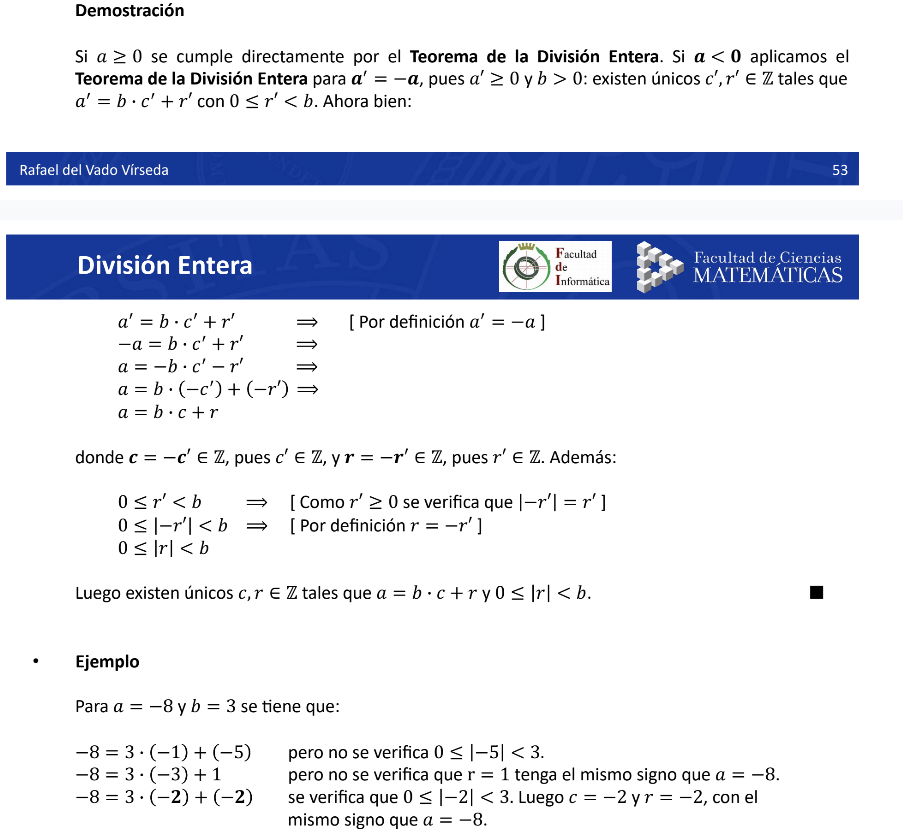
\includegraphics[scale=0.5]{corolario 1}
\end{center}

\item Para $a,b\in \mathbb Z : b>0, \exists! c,r\in \mathbb Z$ que $a:a=bc+r\wedge 0\leq r<b$
\begin{center}
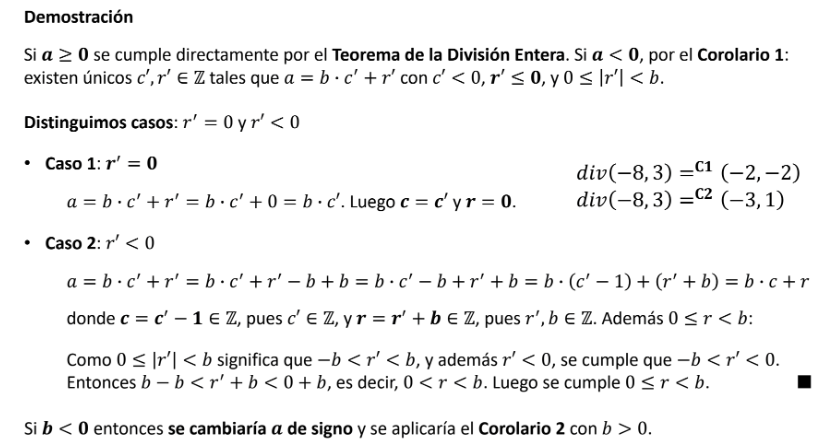
\includegraphics[scale=0.55]{corolario 2}
\end{center}

\item Para $a,b\in \mathbb Z : b\neq 0, \exists! c,r\in \mathbb Z$ que $a:a=bc+r\wedge 0\leq r<b$
\end{itemize}

\subsection*{Múltiplos y divisores}
\subsubsection*{Notación y propiedades}
\begin{itemize}
\item Para decir que \textbf{$a$ es divisor de $b$}: $a\mid b$
\item Para decir que \textbf{$a$ es múltiplo de $b$}: $a\dot{b}$
\item Para decir que $a$ no es divisor de $b$: $a\nmid b$
\item $a\mid b$ y $a\mid n\Rightarrow a\mid (m+n)$ y $a\mid (m\cdot n)$
\item $a\mid m\Rightarrow a\mid m\cdot k$
\item $a\mid m\Rightarrow a\cdot k\mid m\cdot k$
\item $a\mid m\Rightarrow \frac{a}{k}\mid \frac{m}{k}, \forall k\in \mathbb Z$
\end{itemize}
\textbf{\underline{Casos especiales}}:
\begin{itemize}
\item $\frac{0}{0}$ no está definido
\item $0\mid 0$ porque $0=0\cdot 0$
\item $0\nmid a$ con $a\neq 0$ pues no se cumple $a=0\cdot c$
\item $\frac{a}{0}$ no está definido
\end{itemize}

\subsection*{\underline{Teorema de Euclides}}
\subsubsection*{Máximo común divisor}
\begin{itemize}
\item $mcd(0,0)$ no existe
\item $mcd(a,b)=mcd(b,a)$
\item $mcd(a,b)=mcd(|a|,|b|)$
\item $mcd(a,0)=mcd(0,a)=|a|$
\end{itemize}

\subsubsection*{Lema de Euclides}
$$mcd(a,b)=mcd(b,r): a\geq b>0$$
\underline{Demostración}:
\begin{itemize}
\item ``$\subseteq$'' Vamos a ver que todo divisor común de $a$ y $b$ también lo es de $b$ y $r$. $\mbox{Sean }a=d\cdot c_1, b=d\cdot c_2$:
$$r=a-bc=d\cdot c_1-d\cdot c_2\cdot c=d(c_1-c_2-c)\Rightarrow d\mid r$$

\item ``$\supseteq$'' Vamos a ver que todo divisor común de $r$ y $b$ también lo es de $b$ y $a$. $\mbox{Sean }b=d\cdot c_1, r=d\cdot c_2$:
$$a=bc+r=d\cdot c_1\cdot c-d\cdot c_2=d(c_1\cdot c+c_2)\Rightarrow d\mid a$$
\end{itemize}
De este razonamiento se desprende el que $mcd(a,b)=mcd(b,r)$

\subsubsection*{Teorema de Euclides}
Dados $a,b\in \mathbb Z: a>b\geq 0\Rightarrow \exists! mcd(a,b)$\par
\underline{Demostración}:

\begin{enumerate}
\item Demostramos la \textbf{existencia} por inducción completa sobre $b\geq 0$:\par
	Caso base: $b=0$
	$$mcd(a,b)=mcd(a,0)=|a|=a$$
	Paso inductivo, probamos los valores $b>0$:
	$$\mbox{H.I.}\rightarrow \forall b>0: \exists! mcd(a,l): 0\leq l<b \wedge a>l\geq 0$$
	$$a=bc+r$$
	Como $0\leq r<b$ por el teorema de la división entera, podemos tomar como $l=r$ y entonces se verifica $mcd(b,r)$ que por el lema de euclides se extiende a $mcd(a,b)$
	
\item Demostramos ahora la unicidad, por reducción al absurdo:
Supongamos que $d_1=mcd(a,b)$ y $d_2=mcd(a,b)$, con $d_1\neq d_2$ y $d_1,d_2>0$. Por definición de máximo común divisor:
$$
\begin{cases}
d_1\mid d_2\Leftrightarrow d_2=c\cdot d_1 \\
d_2\mid d_1\Leftrightarrow d_1=c'\cdot d_2 
\end{cases}\Rightarrow d_1=c'\cdot d_2=c'\cdot c\cdot d_1\Rightarrow c'\cdot c=1\Leftrightarrow c'=c=1
$$
Luego $d_1=c'\cdot d_2=d_2$ y $d_2=c\cdot d_1=d_1$
\end{enumerate}

\subsubsection*{Algoritmo de Euclides}
Es el algoritmo cuyo objetivo es automatizar la búsqueda de un $mcd(a,b)$ tales que $a\geq b>0$:
\begin{enumerate}
\item Comenzamos dividiendo ambos números:
$$a=b\cdot a_1+ b_1$$
\item Suponemos dos casos:
	\begin{itemize}
	\item $b_1=0$, por el Lema de Euclides:
	$$mcd(a,b)=mcd(a_1,b_1)=mcd(a_1,0)=a_1$$
	
	\item $b_1>0$, entonces tomamos como nuevos $a=a_1$ y $b=b_1$:
	$$a_1=b_1\cdot a_2 + b_2$$
	Y de nuevo llegamos a la tesitura de evaluar si $b_2=0$
	\end{itemize}
\item Con lo cual, dividimos divisor y restos sucesivos, hasta llegar a un momento en el que: $b_i=0$ que significará que:
$$mcd(a,b)=mcd(a_i,b_i)=mcd(a_i,0)=a_i$$
\end{enumerate}
De este modo podemos calcular sin problemas el $mcd(a,b)$ mediante divisiones enteras sucesivas.

\subsection*{\underline{Teorema de Bezout}}
Este teorema dice que elegidos dos números cuales quiera, su máximo común divisor se puede escribir como combinación lineal de cada número por una constante, llamamos a su $mcd(a,b)=d$:
$$d=m\cdot a + n\cdot b$$
Además estos $u$ y $v$ no tienen por qué ser únicos.\par
	
\underline{Demostración}:
Es suficiente con probarlo para $a\geq b>0$, por que en los casos en los que haya negativos, se puede pasar ese signo a $u$ o $v$. Para $a=b=0\Rightarrow \nexists d$, y para $a=b>0\Rightarrow d=a\Rightarrow a=a\cdot 1+b\cdot 0$.\par

Razonamos por inducción completa sobre $b\geq 0$:
\begin{enumerate}
\item Caso base: $b=0$
$$d=mcd(a,b)=mcd(a,0)=a\Rightarrow u=1, v=0$$

\item Paso inductivo, razonamos para $b>0$:
$$\mbox{H.I.} \rightarrow \forall b >0: 0\leq l <b\mbox{ y que } a'>l\geq 0,\mbox{ que si }d'=mcd(a',l)\Rightarrow \exists m',n'\in \mathbb Z: d'=m'a'+n'l$$
Podemos suponer por el teorema de la división entera que $a=bc+r$ y además por el lema de euclides que:
$$mcd(a,b)=mcd(b,r)\stackrel{H.I.}{=}m'b+n'r=m'b+n(a-bc)=n'a+m'b-n'bc	=an'+b(m'-n'c)=am+bn$$
\end{enumerate}

\subsubsection*{Algoritmo de Bezout}
Para calcular los coeficientes mencionados antes que satisfacen la igualdad de Bezout, existe un algoritmo muy sencillo.
\begin{enumerate}
\item Consideramos los primeros $m_k=0$ y $n_k=0$, siendo este $k$ el último paso del algoritmo de Euclides.

\item Tomamos el resto de pares como:
$$m_i=n_{i-1}$$
$$n_i=m_{i-1}-m_i\cdot c_i$$
Donde $c_i$ es el cociente de dicho paso

\item Los valores $m=m_0$ y $n=n_0$ son los correctos.
\begin{center}
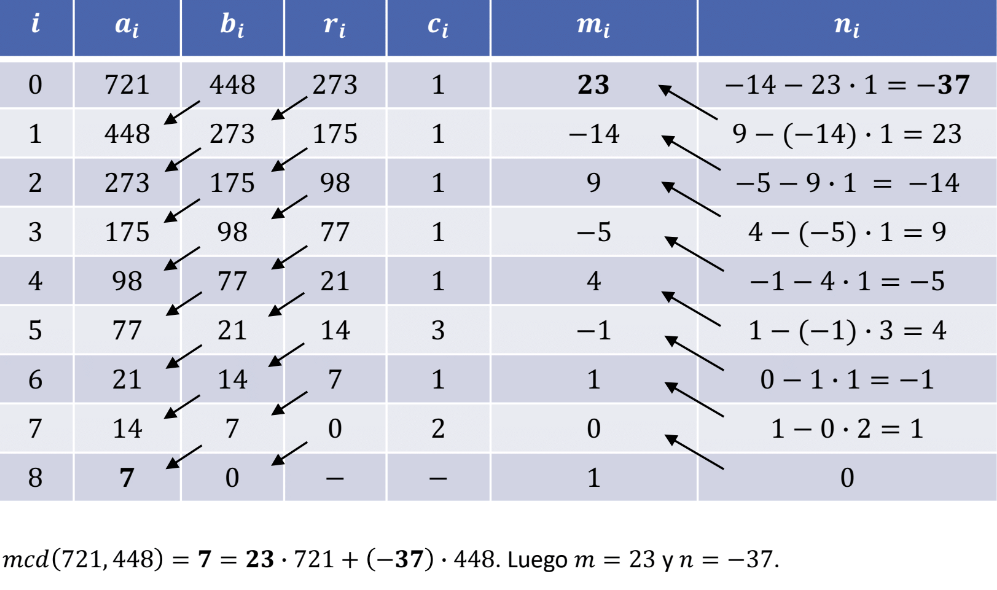
\includegraphics[scale=0.45]{algoritmo de Bezout}
\end{center}
\end{enumerate}

\subsection*{\underline{Mínimo común múltiplo}}
Dados $a,b\in \mathbb Z$ definimos el mínimo común múltiplo de $a$ y $b$ como el menor de los múltiplos comunes.
$$mcm(a,b)=m\Leftrightarrow
\begin{cases}
a\mid m \wedge b\mid m \\
\forall m'\in \mathbb Z: a\mid m' \wedge b\mid m'\Rightarrow m\mid m'
\end{cases}
$$

\subsubsection*{Propiedades:}
\begin{itemize}
\item $mcm(0,0)=0$
\item $mcm(a,b)=mcm(|a|,|b|)$
\item $mcm(a,b)=mcm(b,a)$
\item $mcm(a,0)=0$
\item $mcd(a,b)\cdot mcm(a,b)=a\cdot b: \forall a,b>0$
\end{itemize}

\subsection*{\underline{Números primos}}
Decimos que un número es primo cuando el único divisor además del 1 es sí mismo.
$$p\mbox{ primo}\Leftrightarrow \nexists d\in \mathbb Z: (0<d<p)\wedge d\mid p\Rightarrow \forall d\in \mathbb Z: (d\mid p\Rightarrow d=1\vee d=p)$$
Los números que no son primos son compuestos\footnote{Por convenio, $0$ y $1$ no son primos} y se pueden expresar como producto de primos.

\subsubsection*{Algoritmo para el cálculo de números primos}
Lo que hacemos es seguir el siguiente procedimiento:
\begin{enumerate}
\item Calcular la raíz cuadrada aproximada por truncamiento del número en cuestión.
\item Indicar todos los números primos menores o iguales que esa raíz aproximada. Es decir, busco $0<p^2\leq n$.
\item Si cada uno de los primos indicados anteriormente NO divide a $n$ entonces ese $n$ es primo.\par
Ej.: $n=467$ es primo?
$$\sqrt{467}\simeq 21\Rightarrow 0<p\leq 21\Rightarrow p=2,3,5,7,11,13,17,19$$
Como no hay ningún primo $p: p\mid 467\Rightarrow 467$ es primo.
\end{enumerate}

\subsubsection*{Teorema Fundamental de la Aritmética}
Todo número entero se puede descomponer como producto de primos.
$$\forall n\in \mathbb Z: n=p_1\cdot ...\cdot p_n: p_i\mbox{ es primo}$$
\underline{Demostración}:
\begin{itemize}
\item Existencia: razonamos por reducción al absurdo.
$$n=1\rightarrow 1=p_1^{n_1}\cdot ... \cdot p_m^{n_m}: m=0$$
Demostrado el caso base suponemos para cualquier $k>1$ que se cumple la proposición $P(k)\equiv \forall l\in \mathbb N: 1\leq l<k$, $l$ admite una descomposición en primos. Distinguimos ahora dos casos:
	\begin{itemize}
	\item $k$ es primo:
	$$k=k\cdot 1$$
	
	\item $k$ no es primo:
	$$k=l_1\cdot l_2=p_1^{n_1}\cdot ... \cdot p_m^{n_m}\cdot q_1^{t_1}\cdot ... \cdot q_s^{t_s}$$
	\end{itemize}
	
\item Unicidad: por inducción sobre $t$:
\begin{itemize}
	\item Probamos los casos base: $t=1\Rightarrow p_1=q_1$

	\item Demostrados los casos $n\leq t-1$, demostramos que:
$$p_1\cdot p_2 \cdot ... \cdot p_t=q_1\cdot q_2 \cdot ... \cdot q_s \Rightarrow p_1\mid q_1\cdot ... \cdot q_n\Rightarrow p_1\mid q_i \Rightarrow q_1=p_1\cdot k \Rightarrow k=1\mbox{ por ser primos}$$
	
	Sustituyendo en la expresión inicial:
$$p_1\cdot ... \cdot p_t=p_1\cdot q_2\cdot ... \cdot q_s\Rightarrow p_2\cdot ... \cdot p_t=q_2\cdot ... \cdot q_s$$

	En el primer lado de la igualdad hay $t-1$ factores y en el lado derecho $s-2$, con lo cual:
$$r-1=s-1\stackrel{H.I:}{\Rightarrow }r=s$$
\end{itemize}
\end{itemize}

\subsubsection*{Infinitud de los números primos}
Existen infinitos números primos, aunque no los conozcamos todos.\par
\underline{Demostración}:\par
Sean $p_1,p_2,..., p_n$ los únicos números primos donde $n\in \mathbb N$, escojamos el número:
$$b=p_1\cdot p_2\cdot ... \cdot p_n+1$$
Como $b\notin P=\{p_i: p \mbox{ primo}\wedge i\in \mathbb N\}$, entonces $\exists p_i\in P: b=p_i\cdot c$. Por lo tanto:
$$b=p_1\cdot p_2\cdot ...\cdot p_i \cdot ... \cdot p_n+1\Leftrightarrow 1=p_i\cdot (c- p_1\cdot p_2,...,p_n)\Rightarrow p_i\mid 1\Rightarrow p_i=1\Rightarrow b \mbox{ primo \#}$$

\chapter*{TEORÍA DE CONJUNTOS}
\section*{CONJUNTOS}
Un conjunto es una colección de objetos que está definido de forma clara para saber si un elemento\footnote{El conjunto que contiene a todos los elementos es el \textbf{universal $U$} y el que no contiene a ninguno es el \textbf{vacío $\emptyset$}} pertenece o no a ese conjunto. A los elementos que pertenecen a un conjunto se les denomina \textbf{elementos}.
$$a\in A=\{a\}$$

\subsection*{\underline{Relaciones de pertenencia}}
\begin{itemize}
\item \textbf{Igualdad de conjuntos}: $A=B\Leftrightarrow x\in A\Leftrightarrow x\in B\Leftrightarrow A\subset B\wedge B\subset A$
\item \textbf{Pertenencia o no a un conjunto}: $a\in A=\{x: P(x)\}\Leftrightarrow P(a)\equiv True$
\item \textbf{Inclusión de conjuntos}: $A\subset B\Leftrightarrow \forall a\in A\Rightarrow \forall a\in B$
\end{itemize}

Es decir, si un conjunto contiene a otro, los elementos del primero están contenidos en el segundo y si un elemento pertenece a un conjunto, se encuentra entre sus elementos, \textbf{NO entre los elementos de un conjunto que sea elemento del conjunto mayor}.\par
Ej.:\par

\begin{center}
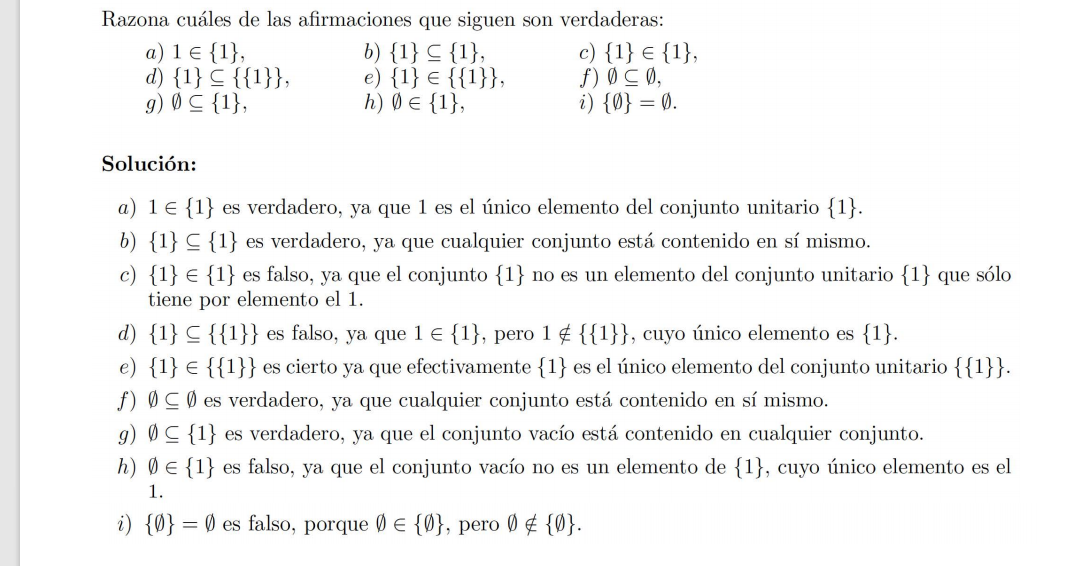
\includegraphics[scale=0.60]{Ejemplo 1}
\end{center}

\begin{center}
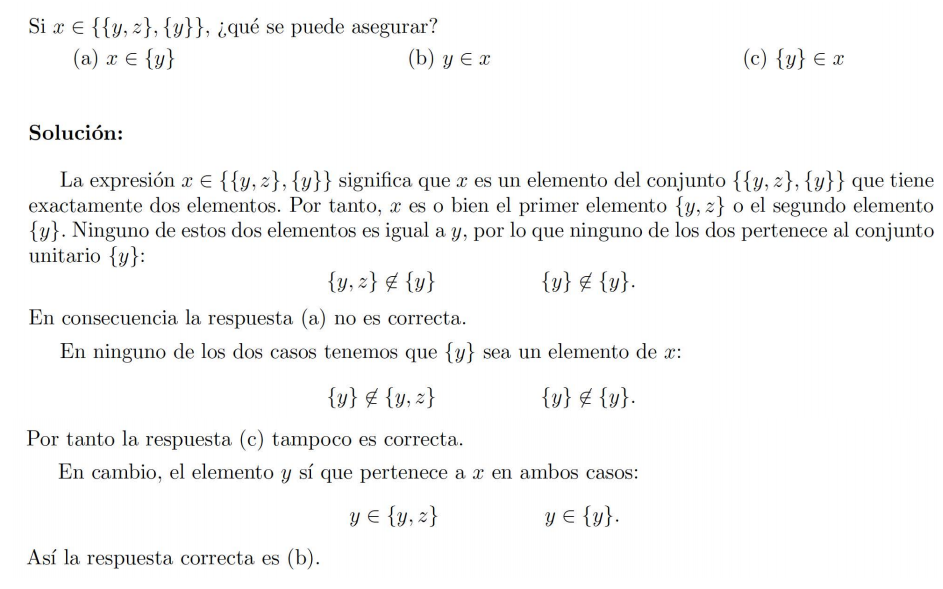
\includegraphics[scale=0.65]{Ejemplo 2}
\end{center}

\subsection*{\underline{Axiomas de la teoría de conjuntos}}
Durante la historia ha habido conflictos lógicos en cuanto a la definición de conjuntos que desmoronaron los cimientos de las matemáticas como la \textbf{paradoja de Rusell}, por ello se fundamento la nueva teoría de conjuntos, \textbf{la axiomática} en lo que se conoce como los \textbf{AXIOMAS DE LA TEORÍA DE CONJUNTOS}:
\begin{itemize}
\item \textbf{Axioma de extensionalidad}: Dos clases $A$ y $B$ que poseen los mismos elementos son la misma clase.

\item \textbf{Axioma del formador de clases}: Para cada fórmula $f(x)$ existe al menos una clase formada por todos los conjuntos que satisfacen la fórmula $f(x)$.

\item \textbf{Axioma del par no ordenado}: El par formado por dos conjuntos es a su vez, otro conjunto.

\item \textbf{Axioma de regularidad}: Para cada clase no vacía, siempre hay al menos un elemento que no contiene otros elementos de la clase, esto es , que es disjunto con ella.

\item \textbf{Axioma de la gran union}: Si $A$ es un conjunto, entonces $\bigcap_{a\in A} a$ es también un conjunto.

\item \textbf{Axioma del conjunto vacío}: $\emptyset$ es el conjunto sin elementos.

\item \textbf{Axioma de infinidad}: Existe un conjunto $A$ con las siguientes propiedades: $\emptyset\in A$ y si $x\in A\Rightarrow x\cup \{x\}\in A$, lo que asegura la existencia de conjuntos infinitos.

\item \textbf{Axioma funcional}: Sea $A$ un conjunto y $f: A\rightarrow B$ una aplicación, entonces $B$ es un conjunto, es decir, si el conjunto del dominio es un conjunto, el conjunto formado por los valores del codominio también lo es para poder establecer la relación entre ambos.

\item \textbf{Axioma del conjunto de partes}: Para cada conjunto $A$ existe un conjunto $P(A)$ formado por todos los subconjuntos de $A$.

\item \textbf{Axioma de Elección}: Dada cualquier familia no vacía de conjuntos no vacíos, dos a dos disjuntos, existe, por lo menos, un conjunto que contiene un elemento y sólo uno de cada conjunto perteneciente a la familia.
\end{itemize}

\subsection*{\underline{Operaciones con conjuntos}}
\begin{itemize}
\item Inclusión: $A\subset B \Leftrightarrow \forall x \in A \Rightarrow x \in B$
\item Equivalencia: $A \equiv B \Leftrightarrow A \subset B \wedge B \subset A$
\item Pertenencia: $x \in A \Leftrightarrow A=\{...,x,...\}$
\item Conjunto vacío: $\emptyset=\{\}: \forall x \in \emptyset$
\item Intersección: $A \cap B=\left\lbrace x: x\in A \wedge x\in B \right\rbrace$
\item Unión: $A \cup B=\left\lbrace x: x\in A \vee x\in B \right\rbrace$
\item Complemento: $A \mbox{\textbackslash} B=\left\lbrace x: x\in A \wedge x\notin B \right\rbrace$
\item Intersecciones múltiples: Sea $I$ un conjunto de de índices y $\forall i \in I$
$$\bigcap_{i\in I}A_i=\left\lbrace x: \forall i \in I : x\in A_i\right\rbrace$$
\item Uniones múltiples: Sea $I$ un conjunto de de índices y $\forall i \in I$
$$\bigcup_{i\in I}A_i=\left\lbrace x: \exists i \in I: x\in A_i\right\rbrace$$
\end{itemize}

\subsubsection*{Familia de Conjuntos}
Cuando a un conjunto no pertenece un elemento sino que más conjunto, decimos que este es una \textbf{familia de conjuntos}. Para este concepto definimos la unión y la intersección como:
$$\bigcup F=\{x: x\in C\mbox{ para algún }C\in F\}$$
$$\bigcap F=\{x: x\in C\mbox{ para todo }C\in F\}$$
Ej.: Sea $M_k=\{n\cdot k: n\in \mathbb N\}$ y $F\{M_k: k\geq2\}=\{M_2,M_3, ...\}$ se define:
$$\bigcup F=\bigcup_{k\geq 2}M_k=\mathbb N\mbox{\textbackslash}\{1\}$$
$$\bigcap F=\bigcap_{k\geq 2}M_k=\{0\}$$

\subsubsection*{Partes de un Conjunto}
Sea A un conjunto, se le llama \textit{partes de A} o P(A) al conjunto formado por todos los subconjuntos de A:
$$\mbox{Ej.: } A=\{a,b,c\}\rightarrow P(A)=\left\lbrace \{a\}, \{b\},\{c\}, \emptyset, \{a,b\}, \{a,c\}, \{b,c\}, A \right\rbrace$$

\subsubsection*{Producto Cartesiano}
Sean A y B conjuntos no vacíos, llamamos par ordenado a una pareja donde $a \in A$ y $b \in B$:
$$(a,b)\neq (b,a) : a\in A \wedge b\in B$$

El producto cartesiano\footnote{Es distributivo con respecto de la unión e intersección de conjuntos} de dos conjuntos es el conjunto:
$$A\times B=\left\lbrace (a,b) : a \in A \wedge b \in B\right\rbrace$$

Dada una colección arbitraria de conjuntos $A_1,A_2,...,A_n$, llamaremos producto cartesiano de los mismos a las n-tuplas ordenadas $(a_1,a_2, ..., a_n)$, donde $a_i\in A_ 1\leq i\leq n$:
$$\underbrace{A\times A\times ... \times A}_{n\mbox{ veces}}=\{(a_1, ..., a_n): a_i\in A, 1\leq i\leq n\}$$

Y se denota por $A^n$

\subsection*{\underline{Álgebra de Boole}}
Si $T$ es un conjunto fijado y $A,B\subseteq T$ dos subconjuntos de T, tenemos que $A\cap B, A\cup B, A\mbox{\textbackslash}B$ y $T\mbox{\textbackslash}A$ son subconjuntos de T.\par
Si $A,B\in P(T)$, entonces como $A\cup B, A\cap B, T\mbox{\textbackslash} A\in P(T)$, podemos definir estos conjuntos como operaciones en $P(T)$.

\subsubsection*{Complementario de un Conjunto}
Dado un conjunto $A\in T$, definimos el complementario como $T\mbox{\textbackslash}A$ y se denota como $\bar{A}$ o \textbackslash$A$

\subsubsection*{Leyes del Álgebra de Boole}
\begin{center}
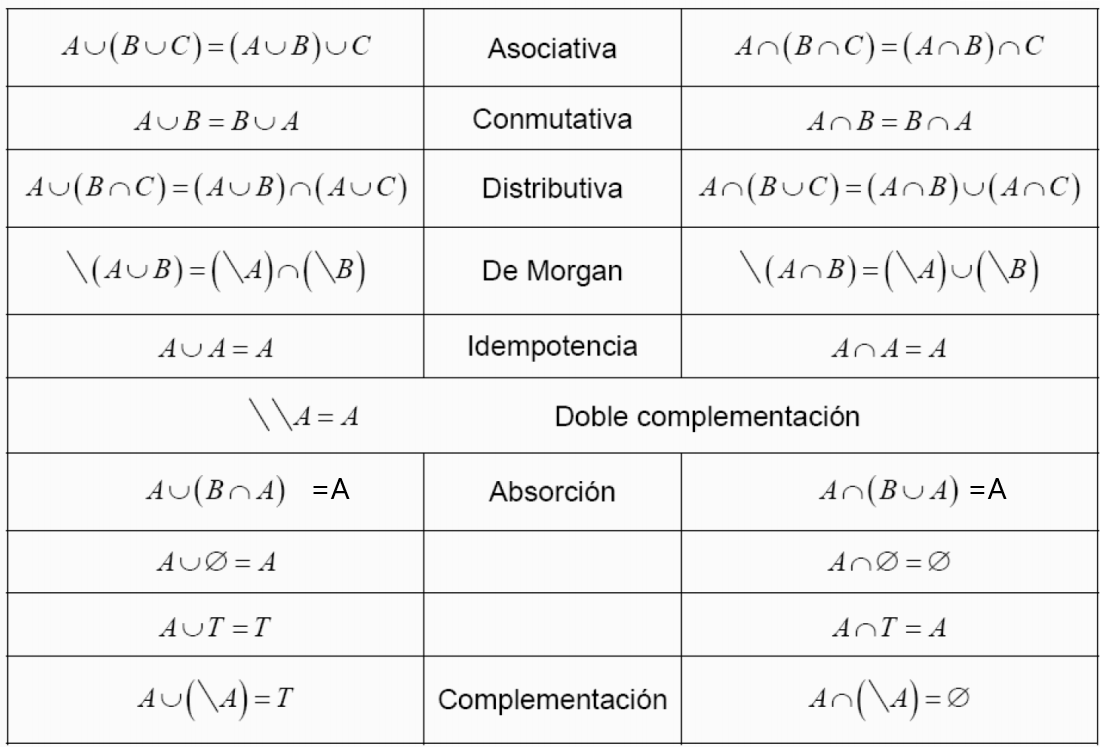
\includegraphics[scale=0.45]{leyes de boole}
\end{center}

Además se le pueden aplicar a este tipo de conjuntos las Leyes de De Morgan vistas en el capítulo de LÓGICA DE PREDICADOS.

\begin{center}
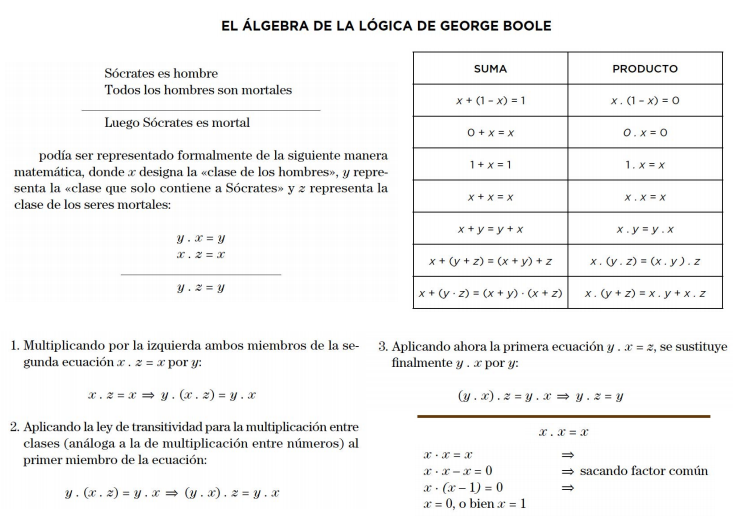
\includegraphics[scale=0.75]{boole articulo}
\end{center}

\section*{RELACIONES BINARIAS}
Una relación binaria es una relación entre dos conjuntos, que a su vez es subconjunto del producto cartesiano de los conjuntos que relaciona.

\begin{center}
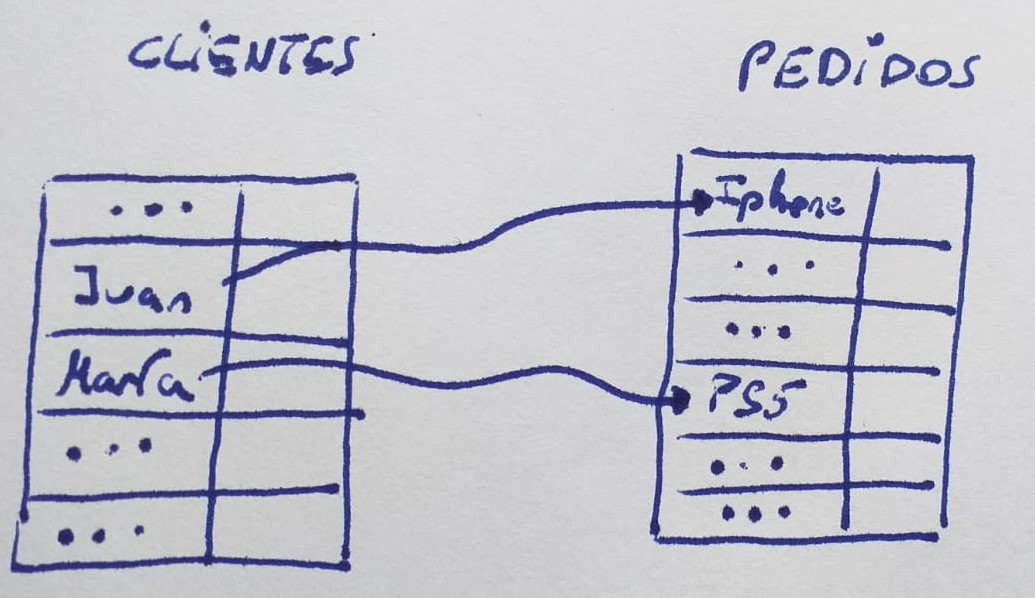
\includegraphics[scale=0.25]{ejemplo relaciones}
\end{center}

$$R=\{(Juan, Iphone 12), (Maria, PS5)\}\subseteq CLIENTES\times PEDIDOS$$
$$S=\{(Juan, Iphone 12,12000€), (Maria, PS5, 3004€)\}\subseteq CLIENTES\times PEDIDOS\times CUENTAS$$

Definimos el concepto de relación binaria entre los conjuntos $A$ y $B$ como un subconjunto $R$ del producto cartesiano de ambos conjuntos: 
$$R\subseteq A\times B$$

Si un par ordenado de los conjuntos de $A$ y $B$ pertenece al conjunto formado por la relación binaria, entonces decimos que $xRy$ y en caso contrario decimos que $x\cancel{R}y$.\par

Definimos el dominio de la relación binaria como:
$$dom(R)=\{x\in A: xRy: \exists y \in B\}$$
Y definimos su imagen o rango como:
$$ran(R)=\{y\in B: xRy: \exists x\in A\}$$\par

Veamos algunos ejemplos de lo comentado anteriormente:
\begin{itemize}
\item Sea $A=\{3,4,5,6\}$ y $B\{2,3,4,5\}$ y $R\subseteq A\times B$
$$xRy\stackrel{Def.}{\Leftrightarrow} x\leq y: \forall x\in A \wedge \forall y\in B\Rightarrow R=\{(3,3), (3,4), (3,5), (4,4), (4,5), (5,5)\}$$
$$dom(R)=\{3,4,5\}\wedge ran (R)=\{3,4,5\}$$

\item Sea $A=B=\{1,2,3,4\}$ y $R\subseteq A^2$:
$$xRy\stackrel{Def.}{\Leftrightarrow}x^2\geq y: \forall x,y\in A$$
Para este ejemplo nos podemos ayudar de un grafo que haga visibles las relaciones entre elementos a través de nodos y líneas de unión:

\begin{center}
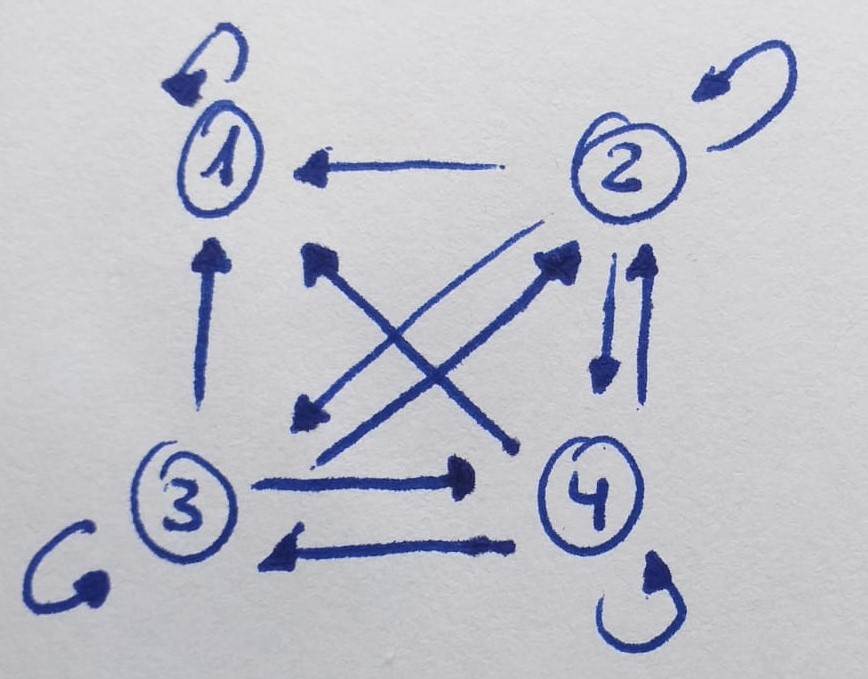
\includegraphics[scale=0.15]{ejemplo 2 relaciones}
\end{center}

$$dom (R)=\{1,2,3,4\}\wedge ran (R)=\{1,2,3,4\}$$

\item Sea $A=B=\{2,3,4,6\}$ y $R\subseteq A^2$:
$$xRy\stackrel{Def.}{\Leftrightarrow} x\mid y: \forall x,y\in A$$
$$dom(R)=A\wedge ran (R)=A$$

\item Sea $A=B=\mathbb R$ y $R\subseteq R^2$:
$$xRy\stackrel{Def.}{\Leftrightarrow} |x|+|y|=1: \forall x,y\in \mathbb R$$
$$dom(R)=[-1,1]\wedge ran (R)=[-1,1]$$
\end{itemize}

\subsubsection*{Propiedades de las relaciones binarias}
Sea $R\subseteq A^2$, esta cumple las siguientes propiedades:
\begin{itemize}
\item \textbf{Reflexiva}: $\forall x \in A: xRx$
\item \textbf{Antireflexiva}: $\nexists x\in A: xRx$
\item \textbf{Simétrica}: $\forall x,y \in A: xRy\Rightarrow yRx$
\item \textbf{Antisimétrica}: $\forall x,y \in A: (xRy\wedge yRx)\Rightarrow x=y$
\item \textbf{Transitiva}: $\forall x,y,z \in A: (xRy\wedge yRz)\Rightarrow xRz$
\item \textbf{Conexa}: $\forall x,y\in A: x\neq y\Rightarrow (xRy\vee yRx)$
\end{itemize}

Veamos algunos ejemplos:
\begin{itemize}
\item Sea $A=\mathbb N\mbox{\textbackslash}\{0\}$ y $R\subseteq A^2$
$$xRy\stackrel{Def.}{\Leftrightarrow} mcd(x,y)=1: \forall x,y\in A$$
	\begin{enumerate}
	\item reflexividad: $xRx: \forall x \in A$?
	$$mcd(x,x)=1: \forall x\in A\Rightarrow \#\Rightarrow NO$$
	\item antireflexividad: $\nexists x\in A: xRx$?
	$$\nexists x\in A: mcd(x,x)=1\Rightarrow \# \Rightarrow NO$$
	\item simetría: $\forall x,y \in A: mcd(x,y)=1\Rightarrow mcd(y,x)=1$?
	$$mcd(x,y)=mcd(y,x)=1\Rightarrow SI$$
	\item antisimetría: $\forall x,y \in A: mcd(x,y)=mcd(y,x)=1\Rightarrow x=y$?
	$$mcd(a,b)=mcd(b,a)=1: \mbox{a y b primos}\nRightarrow a=b\Rightarrow NO$$
	\item transitividad: $\forall x,y,z \in A: mcd(x,y)=1=mcd(y,z)\Rightarrow mcd(x,z)=1$?
	$$mcd(4,7)=1=mcd(7,2)\mbox{ , pero }mcd(4,2)\neq 1\Rightarrow NO$$
	\item conexión: $\forall x,y \in A: x\neq y\Rightarrow mcd(x,y)=1 \vee mcd(y,x)=1$?
	$$2\neq 4, mcd(2,4)=1\wedge mcd(4,2)\neq 1\Rightarrow NO$$
	\end{enumerate}
\end{itemize}

\subsection*{\underline{Operaciones entre relaciones binarias}}
Sean $R$ y $S$ dos relaciones tal que $R,S\subseteq A\times B$ y la relación binaria $T\subseteq B\times C$.
\begin{itemize}
\item \textbf{Relación Unión}: $R\cup S=\{(x,y)\in A\times B: xRy \vee xSy\}$

\item \textbf{Relación Intersección}: $R\cap S=\{(x,y)\in A\times B: xRy \wedge  xSy\}$

\item \textbf{Relación Complemento}: $\overline{R}=\{(x,y)\in A\times B: xRtachadoy\}$

\item \textbf{Relación Inversa}: $R^{-1}=\{(y,x)\in B\times A: xRy\}$

\item \textbf{Relación Composición (o producto)}: $R\cdot S=\{(x,z)\in A\times C:\exists y\in B: xRy\wedge ySz\}$

\item \textbf{Relación Identidad}: $id_A=\{(x,x)\in A\times A: x\in A\}$
\end{itemize}

\subsubsection*{Propiedad de las operaciones}
Sean $R\subseteq A\times B$, $S\subseteq B\times C$ y $T\subseteq C\times D$
\begin{itemize}
\item \textbf{Asociatividad}: $R\cdot (S\cdot T)=(R\cdot S)\cdot T$

\item \textbf{Elemento neutro}: $id_A\cdot R=R\cdot id_A=R$

\item \textbf{Elemento inverso\footnote{NO es conmutativo}}: $(R\cdot S)^{-1}=S^{-1}\cdot R^{-1}$
\end{itemize}

\underline{Demostración de la 3}:
$$z(R\cdot S)^{-1}x\Leftrightarrow x(R\cdot S)z\Leftrightarrow \exists y: xRy\wedge ySz\Leftrightarrow \exists y: yR^{-1}x \wedge zS^{-1}s\Leftrightarrow \exists y: zS^{-1}y\wedge yR^{-1}x\Leftrightarrow z(S^{-1}\cdot R^{-1})x$$

\section*{FUNCIONES}
Las funciones son relaciones binarias. Una relación binaria , $R\subseteq A\times B$, es una función si para todo $a\in A$ existe \textbf{a lo sumo} un $b\in B$ tal que $aRb$:
$$\forall a \in A: (\exists! b\in B: aRb)\vee (\nexists b\in B: aRb)$$
Por ejemplo, $R\subseteq Z\times Z: xRy\stackrel{def}{\Leftrightarrow} y=x^2$, sí es una función porque $\forall x\in \mathbb Z: \exists! y\in \mathbb Z: xRy$, pero la función inversa $xR^{-1}y\Leftrightarrow x=y^2\Leftrightarrow y=\sqrt{x}$, no es función porque hay puntos del dominio que tienen más de una imagen.

\subsubsection*{Notación, dominio y rango y concepto de función total}
Por \textbf{notación}, escribiremos $y=f(x)$, donde $f:A\rightarrow B$, para referirnos a la relación binaria a la que llamamos función e indicar los conjuntos que relaciona.\par
Al \textbf{dominio} y al \textbf{rango} los denotaremos como:
\begin{itemize}
\item $dom (f)=\{x\in A: \exists f(x)\}\subseteq A$
\item $ran (f)=\{f(x)\in B: x\in dom (f)\}\subseteq B$
\end{itemize}

Una función $f: A\rightarrow B$ es \textbf{total} si $dom(f)=A$, por el contrario, $f: A\cancel{\longrightarrow}B$ es \textbf{parcial}\footnote{También se usa la notación de $f: A \dashrightarrow B$} si $dom(f)\subset A$.

\subsection*{\underline{Operaciones con funciones}}
Definimos las siguientes operaciones:
\begin{enumerate}
\item \textbf{Restricción de $f:A\rightarrow B$ a $C\subseteq A$}:
\begin{itemize}
\item $f\mid_C: C\rightarrow B$
\item $f\mid_C(x)=f(x): \forall x\in dom(f)\cap C$
\end{itemize}

\item \textbf{Composición de $f:A\rightarrow B$ y $g:B\rightarrow C$}:
\begin{itemize}
\item $f\circ g: A\rightarrow C$
\item $f\circ g(x)=g(f(x))\Rightarrow \begin{cases}dom(f\circ g)=\{x\in dom(f): f(x)\in dom(g)\}\\ ran(f\circ g)=\{ran(g\mid_{dom(g)\cap ran(f)})\}\end{cases}$
\end{itemize}

\item Inversa de una función $f: A\rightarrow B$:
\begin{itemize}
\item $f^{-1}=B\rightarrow A$
\item $f^{-1}(x)=y\Leftrightarrow f(y)=x$
\end{itemize}
\end{enumerate}

\subsubsection*{Propiedades de las operaciones}
Sean $f:A\rightarrow B$, $g: B\rightarrow C$ y $h:C\rightarrow D$:
\begin{itemize}
\item \textbf{Asociativa}: $(f\circ g)\circ h=f\circ(g\circ h)$
\item \textbf{Elemento inverso\footnote{$id_A: A\longrightarrow A: id_A(x)=x$ y análogo con $id_B$}}: $f\circ f^{-1}=id_A$ ó $ f^{-1}\circ f=id_B$
\item \textbf{Elemento neutro}: $id_A\circ f=f\circ id_B=f$
\end{itemize}
Que como vemos le otorga a este conjunto junto con la operación composición estructura de cuerpo.

\subsection*{\underline{Propiedades de las funciones}}
\subsubsection*{Inyectividad}
Sean A y B conjuntos y $f: A \rightarrow B$ una función, se dice que $f$ es \textbf{inyectiva} cuando todo elemento de A posee una imagen distinta de la imagen de cualquier otro elemento de A:
$$\forall a_1, a_2 \in A : a_1 \neq a_2\Rightarrow f(a_1)\neq f(a_2)$$

En la práctica, para calcular si una función es inyectiva o no, tomaremos $f(x_1)=f(x_2)$ y si eso resulta en $x_1=x_2$ entonces es inyectiva, si no no.\par

Ej.:  "$f(x)=x^2$"
$$f(x_1)=f(x_2)\Rightarrow x_1^2=x_2^2\Rightarrow x_1^2-x_2^2=0 \Rightarrow$$
$$\Rightarrow (x_1-x_2)(x_1+x_2)=0 \Rightarrow
\begin{cases}
x_1-x_2=0 \Rightarrow & x_1=x_2 \\
x_1+x_2=0 \Rightarrow & x_1=-x_2 \\
\end{cases}
\Rightarrow \mbox{ no es inyectiva}$$

También se puede coger un elemento $y$ que pertenezca a la imagen, despejar $x$ de $y=f(x)$ y ver si para un mismo $y$ hay varios valores de $x$:\par
Ej.: $f: \mathbb R^+ \rightarrow \mathbb R^+ : f(x)=\frac{x^2}{1+x}$
$$y\in im(f)\Rightarrow y=f(x)=\frac{x^2}{1+x}\Leftrightarrow x^2-yx-y=0$$
$$x=\frac{y\pm \sqrt{y^2+4y}}{2}\mbox{ pero como }\frac{y-
 \sqrt{y^2+4y}}{2}<0\Rightarrow x\notin \mathbb R^+\Rightarrow inyectiva$$
Ej.: ``$E=\{x\in \mathbb R : 1\leq x\leq 2\}$, $G=\{y\in \mathbb R : 1\leq y\leq 4\}$ y $f(x)=\frac{1}{x^2}$''
$$f(E)?\rightarrow 1\leq x\leq 2\Leftrightarrow 1\leq x^2\leq 4\Leftrightarrow 1\geq x\geq \frac{1}{4}=f(E)$$
$$f^{-1}(G)?\rightarrow 1\leq y=f(x)=\frac{1}{x^2}\leq 4\Leftrightarrow 1\geq x^2\geq \frac{1}{4}\Leftrightarrow 1\geq |x|\geq \frac{1}{2} 
\begin{cases}
1\geq x\geq \frac{1}{2}& \Rightarrow 1\geq x\geq \frac{1}{2} \\
1\geq -x\geq \frac{1}{2}& \Rightarrow -1\leq x\leq -\frac{1}{2}
\end{cases}$$

\subsubsection*{Suprayectividad}
Sean A y B conjuntos y $f: A \rightarrow B$ una función, se dice que $f$ es \textbf{suprayectiva} o \textit{sobre} cuando todo elemento de B es imagen\footnote{Lo que se traduce en que $im(f)=B$} de algún elemento de A:
$$\forall b \in B : \exists a \in A : f(a)=b$$

En la práctica, para calcular si una función es inyectiva o no, tomaremos $y=f(x)$ y despejaremos $x$, si $y$ toma como posibles valores los mismos que los valores del codominio, es suprayectiva.\par

Ej.:  "$f(x)=x^2$"
$$y=x^2\Rightarrow x=\sqrt{y}\Rightarrow y\in (0,\infty)$$
Luego no es suprayectiva porque $f: \mathbb R \rightarrow \mathbb R$

\subsubsection*{Biyectividad}
Sean A y B conjuntos y $f: A \rightarrow B$ una función, se dice que $f$ es \textbf{biyectiva} cuando $f$ es inyectiva y suprayectiva simultáneamente.\par
Que en el fondo también es decir que $\exists f^{-1}$

\section*{CARDINALIDAD}
Un conjunto $A$ es FINITO si $\exists n\in \mathbb N$ de manera que exista  una biyección entre $\{0,1,...,n-1\}$ y el conjunto que queremos determinar como finito\footnote{Los conjuntos infinitos son aquellos que no son finitos}.\par
En este caso decimos que $n$ es el \textbf{cardinal} de A y se representa como $|A|$.

Ej.: $A,B\subseteq \mathbb N: A,B$ son infinitos, selecciona la opción correcta:
\begin{enumerate}
\item $\mathbb N\mbox{\textbackslash}(A\cup B)$ es finito
\item $A\cap B$ es infinito
\item $A\cup B$ es infinito
\item Ninguna de las anteriores
\end{enumerate}

Consideramos que $A=\{n\in \mathbb N: n\mbox{ es }\dot{3}\}$ y $B=\{n\in \mathbb N: n-1\mbox{ es }\dot{3}\}$, esto implica que $\mathbb N\mbox{\textbackslash}(A\cup B)=\{n\in \mathbb N: n-2\mbox{ es }\dot{3}\}$ que es infinito. $\Rightarrow 1)\#$

Es fácil ver que $A\cup B$ es infinito, luego $3)\Rightarrow Ok$

\subsection*{\underline{Propiedades de los cardinales}}
El concepto de cardinal que estamos tratando SÓLO es aplicable a CONJUNTOS FINITOS:
\begin{itemize}
\item $S\subseteq A\Rightarrow |S|\leq |A|$
\item $|A\cup B|=|A|+|B|-|A\cap B|$
\item $A\mbox{\textbackslash}B=|A|-|A\cap B|$
\item $|A\times B|=|A|\cdot |B|$
\item $|\{f\mid f: A\longrightarrow B\}|=VR_{|B|}^{|A|}=|B|^{|A|}$
\item $|P(A)|=2^{|A|}$
\end{itemize}

\subsubsection*{Principio del Palomar}
Surge de la situación de meter palomas en huecos de un palomar, si tenemos que meter cada paloma en un hueco y vemos que hay más palomas en huecos, necesariamente algún hueco tendrá más de una paloma.\par

Volviendo a las matemáticas, lo que queremos decir es que si:
$$f:A\longrightarrow B\wedge |A|>|B|\Leftrightarrow \nexists f\mbox{ inyectiva}$$

Y además esto quiere decir que hay, al menos, $\frac{|A|}{|B|}$ aproximado al entero superior, número de palomas que comparten hueco.

\subsection*{\underline{Relaciones de Cardinalidad}}
Sean $A$ y $B$ dos conjuntos\footnote{No necesariamente finitos}, entonces son:
\begin{itemize}
\item \textbf{Equipotentes}: $A\sim B \Leftrightarrow \exists f: A\longrightarrow B: f \mbox{ \textbf{biyectiva}}$, es decir, si son finitos, entonces: $|A|=|B|$.\par
Esta relación entre ambos $\sim$ es una RELACIÓN DE EQUIVALENCIA.\footnote{Las características de la relación son reflexividad, simetría y transitividad}

\item \textbf{Dominación}: Se dice que $A$ está dominado por $B$ y se expresa como: $A\leq B\Leftrightarrow \exists f: A\longrightarrow B: f\mbox{ \textbf{inyectiva}}$, es decir, si $A$ y $B$ son finitos, entonces $|A|\leq |B|$.\par
Esta relación entre ambos $\sim$ es una RELACIÓN DE ORDEN.\footnote{Las características de la relación son reflexividad, "antisimetría" y transitividad}\par
\textit{Teorema de Schröeder-Bernstein}:
$$A\leq B \wedge B\leq A\Rightarrow A\sim B$$

\item \textbf{Dominación estricta}: $A$ está estrictamente dominado por $B$ y se expresa como $A<B$, si está dominado, pero no son equipotentes.
\end{itemize}

\subsection*{\underline{Conjuntos numerables y no numerables}}
Decimos que un conjunto es \textbf{numerable} cuando podemos establecer una biyección entre él y los números naturales, es decir, son equipotentes.\footnote{En esta asignatura los conjuntos finitos también los consideramos numerables}.
$$A\mbox{ numerable}\Leftrightarrow A\mbox{ finito }\vee A\sim \mathbb N$$
Como ejemplos vemos que los naturales, los enteros, los racionales, los pares, los impares, los primos, $\mathbb N_m$... son numerables.\par

\textbf{\underline{Propiedades}}:\par
Además, tenemos que si $A_i\sim \mathbb N$, entonces:
\begin{itemize}
\item $\bigcup_{i=1}^m A_i\sim \mathbb N$
\item $\bigcup_{i\in \mathbb N} A_i\sim \mathbb N$
\item $A_1\times A_2\times ...\times A_n\sim \mathbb N$
\end{itemize}

Decimos que un conjunto es \textbf{NO numerable} cuando no se cumplen las premisas de ser numerable.
$$A\mbox{ no numerable}\Leftrightarrow A\mbox{ no es finito }\wedge A\nsim \mathbb N$$

Ej.: Demostrar que $\mathbb N\times \mathbb N \sim \mathbb N$

Para estas demostraciones es útil demostrar que uno es dominante sobre el otro y viceversa.Si tenemos que $f:\mathbb N\times \mathbb N\longrightarrow \mathbb N$ podemos definir la función: $f((n,m))=2^n\cdot 3^m$ y vemos que claramente es inyectiva.

En el otro sentido, si tenemos que $g:\mathbb N \longrightarrow \mathbb N \times \mathbb N$ siendo $g(n)=(n,0)$, vemos claramente que es inyectiva y, en consecuencia, podemos decir que ambos se dominan el uno al otro, lo que implica que son equipotentes.

\subsubsection*{Demostración de la NO numerabilidad de los $\mathbb R$}
Vamos a demostrar que $[0,1)\nsim \mathbb N$ y en consecuencia $\mathbb R \nsim \mathbb N$. Razonamos por reducción al absurdo: supongamos que $[0,1)\sim  \mathbb N\Rightarrow \exists f: [0,1)\longrightarrow \mathbb N: f\mbox{ biyectiva}$

\begin{center}
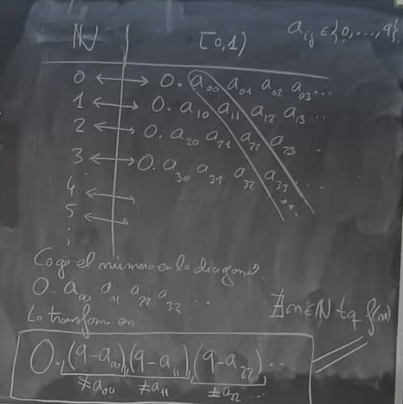
\includegraphics[scale=1.1]{No numerabilidad de R}
\end{center}

Vemos que si podemos establecer una biyección, entonces a cada natural le puede corresponder un número en el intervalo $[0,1)$. Como son reales, tienen infinitos decimales por lo que yo puedo escribirlos como en la imagen siendo $a_{ij}\in \{0, ..., 9\}$ y se relación con los naturales como se muestra en la imagen.\par
Posteriormente, si cogemos la diagonal principal como está rodeada, tenemos que el número formado es el número que se muestra abajo. Si ese número lo transformas de forma que quede la parte encuadrada abajo (que es completamente válido porque sigue siendo un real del intervalo), entonces vemos que este número siempre se diferencia de cada número de la tabla por lo menos en algunas de las cifras. En consecuencia, ya no puede estar emparejado con ninguno de los naturales.


\chapter*{RELACIONES DE \\ EQUIVALENCIA Y ORDEN}

\section*{RELACIONES DE EQUIVALENCIA}
Una relación de binaria $R\subset A\times A$ sobre un conjunto A cualquiera es una relación de equivalencia si es:
\begin{itemize}
\item Reflexiva
\item Simétrica
\item Transitiva
\end{itemize}
Y en ese caso escribimos $X\sim Y$ en lugar de $xRy$.\par
Las relaciones de equivalencia establecen una partición sobre el cuerpo en el que están definidas, dividiendo el mismo en clases de equivalencia y, en consecuencia, haciendo que todos los elemento del cuerpo pertenezcan a una y solo una de las clases de equivalencia definidas.

\subsection*{\underline{Clases de equivalencias}}
Dada una relación de equivalencia ``$\sim$'' sobre un conjunto $A$ y un elemento $x\in A$ perteneciente al mismo, se define como la \textbf{clase de equivalencia} de $x$ como:
$$[x]=\{y\in A: x\sim y\}$$

\subsubsection*{Propiedades}
Definidas las clases de equivalencia, es fácil ver las siguientes propiedades referidas a las mismas:
\begin{itemize}
\item $x\in [x]$
\item $x\sim y\Leftrightarrow [x]=[y]$
\item $x\nsim y\Rightarrow [x]\neq [y]\Rightarrow [x]\cap [y]=\emptyset$
\end{itemize}

Ej.: En $\mathbb Z$, consideramos $xRy\Leftrightarrow x+3y=\dot 4$.:
\begin{itemize}
\item $\mbox{Reflexiva: } xRx\Leftrightarrow x+3x=4 \div 4$
\item $\mbox{Simetrica: } xRy\Rightarrow x+3y=4k \Rightarrow 4\mid x \wedge 4\mid y\Rightarrow y+3x=4k+3\cdot 4\cdot k=4(k+3k)\Rightarrow yRx$

\item Transitiva: fácil de demostrar
\end{itemize}
Con lo cual, la clase de equivalencia $[4]=\{y\in \mathbb Z: 4Ry\}=\{y\in \mathbb Z: 4-3y=4k\}\Rightarrow y=\dot{4}$

\subsection*{\underline{Conjunto cociente}}
Definimos el conjunto cociente denotado por $A/\sim$ como el conjunto de todas las clases que forman los elementos de $A$ con respecto a esa clase de equivalencia.
$$A/\sim\quad =\{[x]: x\in A\}$$

Por ejemplo, tenemos en las relaciones de congruencia $\mathbb Z/n$ donde $\mathbb Z/n=\{[0], [1], ...,[n-1]\}$.\par

Ej.: En $\mathbb N\times \mathbb N$ definimos $(a,b)R(c,d)\Leftrightarrow a+d=b+c$. Vemos que $(0,0)R(1,1)$, $(0,0)R(2,2)R...$, también tenemos que $(1,0)R(2,1)$.

\begin{center}
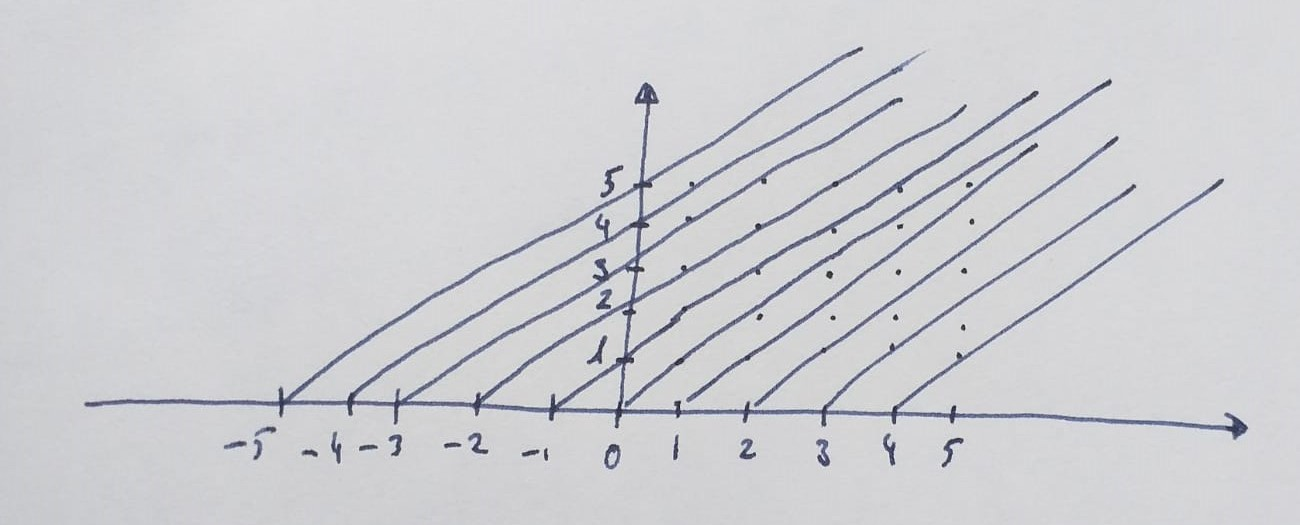
\includegraphics[scale=0.35]{definicion enteros}
\end{center}

Es fácil comprobar que es una relación de equivalencia. Entonces, vemos que si prolongamos dichas rectas, cada clase de equivalencia que corresponde a cada una de las rectas. Se puede definir que $\mathbb N\times \mathbb N/R \sim \mathbb Z$; construyendo así los números enteros.

\section*{RELACIONES DE ORDEN}
\subsection*{\underline{Conjuntos ordenados y relación usual de orden}}
Una relación binaria $R\subset A\times A$ sobre un conjunto $A$ es una \textbf{RELACIÓN DE ORDEN}\footnote{Ordinario o parcial representado por: $\sqsubseteq$} si es:
\begin{itemize}
\item Reflexiva
\item Antisimétrica
\item Transitiva
\end{itemize}

Además, decimos que se trata de una relación de \textbf{ORDEN TOTAL o lineal} si además es:
\begin{itemize}
\item Conexa
\end{itemize}

Llamamos \textbf{CONJUNTO ORDENADO} al par $(A, \sqsubseteq)$ formado por el conjunto $A$ sobre el que está definida la relación de orden $\sqsubseteq$ y la propia relación de orden.
\begin{itemize}
\item Ej.: $(A,\leq )$, siendo $A$ cualquier conjunto contenido en $\mathbb R$ es un conjunto ordenado porque ``$\leq$'' cumple las premisas de relación de orden. Además, constituye un orden total.

\item Ej.: $(\mathbb N_1, \mid)$ también cumple las premisas de conjunto ordenado.

\item $(P(A), \subseteq )$ para cualquier conjunto $A$ y la relación de inclusión usual.
\end{itemize}

\subsection*{\underline{Relación de orden estricto}}
Si tenemos una relación binaria $R\subset A\times A$ sobre un conjunto $A$, decimos que es un \textbf{ORDEN ESTRICTO}\footnote{Representado por $\sqsubset$} si cumple las propiedades:
\begin{itemize}
\item Antireflexiva
\item Transitiva
\end{itemize}

Además, decimos que se trata de una relación de \textbf{ORDEN ESTRICTO TOTAL o lineal} si además es:
\begin{itemize}
\item Conexa
\end{itemize}

\subsection*{\underline{Diagramas de Hasse}}
Sirven para representar gráficamente\footnote{Son útiles para estructuras de datos discretos, por lo que son útiles para conjunto finitos e infinitos numerables porque su representación para conjuntos de mayor cardinal es demasiado compleja y se usan otras estructuras} conjuntos ordenados. Dado un conjunto ordenado $(A,\sqsubseteq)$ su \textit{diagrama de Hasse} se obtiene mediante el siguiente algoritmo:
\begin{itemize}
\item Cada elemento del conjunto $A$ se representa en un vértice

\item Se dibuja una linea en dirección ascendente entre los vértices $x$ e $y$ si $x\sqsubseteq y$ y además no hay ningún elemento entre medias de ellos, es decir, $\nexists z\in A: x\sqsubseteq z \sqsubseteq y$
\end{itemize}

Ej.: Si $A=\{1,2,3,4,6,24\}$ y $\sqsubseteq \sim \mid$, entonces tenemos un conjunto ordenado y su diagrama de Hasse es: 
\begin{center}
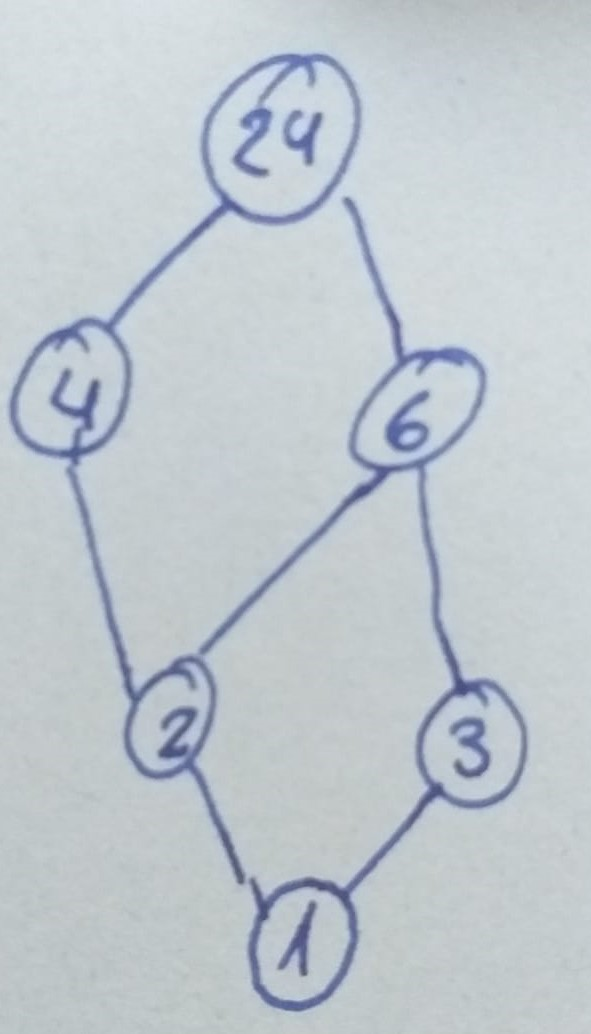
\includegraphics[scale=0.15]{Diagrama de Hasse}
\end{center}

\subsection*{\underline{Elementos especiales de los conjuntos ordenados}}
Sea $(A,\sqsubseteq )$ un conjunto ordenado y $S\subseteq A$:
\begin{itemize}
\item \textbf{ELEMENTOS EXTREMOS}:
	\begin{itemize}
	\item $x\in S$ es el \textbf{máximo} de $S$ si $y\sqsubseteq x: \forall y\in S$
	
	\item $x\in S$ es el \textbf{mínimo} de $S$ si $x\sqsubseteq y: \forall y\in S$
	\end{itemize}
	
\item \textbf{ELEMENTOS EXTREMALES}:
	\begin{itemize}
	\item $x\in S$ es el \textbf{maximal} en $S$ si $\nexists y \in S: x\neq y: x\sqsubseteq y$
	
	\item $x\in S$ es el \textbf{minimal} en $S$ si $\nexists y \in S: x\neq y: y\sqsubseteq x$.
	\end{itemize}
\end{itemize}

Ej.: Consideramos el conjunto ordenado $(A,\mid)$, donde $A=\{1,2,3,4,6\}$. Su diagrama de Hasse es:
\begin{center}
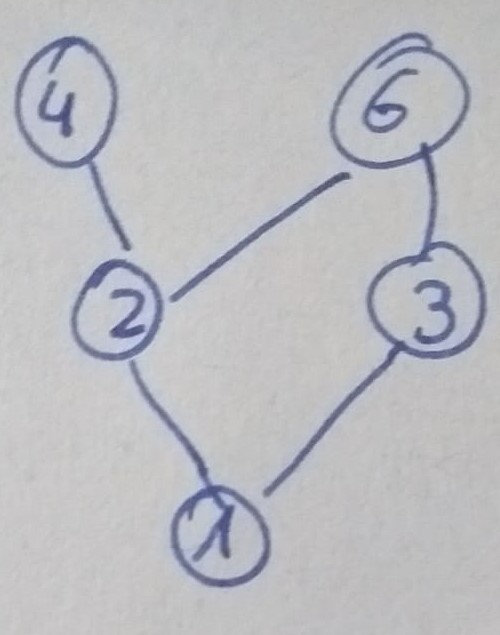
\includegraphics[scale=0.15]{Diagrama de Hasse2}
\end{center}

Sea $S=A$, entonces tenemos que $4$ y $6$ son maximales, pero sin embargo no existe el máximo porque ningún elemento es mayor que TODOS. El único minimal que existe es el 1, que en este caso coincide con el mínimo. Si solo nos fijamos en el segundo nivel, es decir, $S=\{2,3\}$, entonces tenemos que existen dos maximales, ningún maximo y dos minimales, pero ningún mínimo.

Del mismo modo, si $(A,\sqsubseteq)$ un conjunto ordenado y  $S\subset A$:
\begin{itemize}
\item \textbf{COTAS}:
	\begin{itemize}
	\item $x\in A$ es \textbf{cota superior} de $S$ si $u\sqsubseteq x: \forall u\in S$.
Al conjunto de todas las cotas superiores de un conjunto se le denota por:
$$Sup(S)=\{x\in A: x\mbox{ es cota superior de }S\}$$

	\item $x\in A$ es \textbf{cota inferior} de $S$ si $x\sqsubseteq u: \forall u\in S$.
Al conjunto de todas las cotas inferiores de un conjunto se le denota por:
$$Inf(S)=\{x\in A: x\mbox{ es cota inferior de }S\}$$
\end{itemize}

\item \textbf{SUPREMOS E ÍNFIMOS}:
	\begin{itemize}
	\item $x\in A$ es \textbf{supremo} de $S$ si es el mínimo en la relación de orden ``$\sqsubseteq$'' definida del conjunto $Sup(S)$:
	$$\bigsqcup S=\min Sup(S)$$

\item $x\in A$ es \textbf{ínfimo} de $S$ si es el máximo en la relación de orden ``$\sqsubseteq$'' definida del conjunto $Inf(S)$:
	$$\sqcap S=\max Inf(S)$$
\end{itemize}
\end{itemize}

\subsection*{\underline{Funciones que conservan el orden}}
\subsubsection*{Funciones monótonas}
Las funciones que respetan el orden de los elementos a los que se les aplica se llaman \textbf{funciones monótonas}, es decir, sean $(A,\sqsubseteq_A)$ y $(B,\sqsubseteq_B)$ dos conjuntos ordenados y la función $f: A\rightarrow B$:
$$f\mbox{ es monótona} \Leftrightarrow \forall x,y\in A: x\sqsubseteq_A y \Rightarrow f(x)\sqsubseteq_B f(y)$$

\subsubsection*{Funciones que preservan el orden}
Son funciones monótonas en las que si se cumple el recíproco de la propiedad que definía el concepto de función monótona.
$$f\mbox{ conserva el orden} \Leftrightarrow \forall x,y\in A: x\sqsubseteq_A y \Leftrightarrow f(x)\sqsubseteq_B f(y)$$

\subsubsection*{Isomorfismo y automorfismo de orden}
Decimos que una función es un \textbf{isomorfimo de orden} si es una función que conserva el orden y además es biyectiva.\par
Decimos que una función es un \textbf{automorfismo} de orden cuando es un isomorfimo y además el conjunto de llegada y de partida es el mismo.

\subsubsection*{Teorema}
Sean $(A,\sqsubseteq_A)$ y $(B,\sqsubseteq_B)$ dos conjuntos ordenados y la función $f: A\rightarrow B$ un isomorfismo de orden, entonces:
\begin{itemize}
\item $x=\max A\Leftrightarrow f(x)=\max B$
\item $x=\mbox{ maximal en }  A\Leftrightarrow f(x)=\mbox{ maximal en } B$
\item $x=\min A\Leftrightarrow f(x)=\min B$
\item $x=\mbox{ minimal en }  A\Leftrightarrow f(x)=\mbox{ minimal en } B$
\end{itemize}

\chapter*{TEORÍA DE GRAFOS}
\section*{CONCEPTO DE GRAFO Y TIPOS}
\subsection*{\underline{Tipos de grafos}}
\subsubsection*{Grafo no dirigido}
Un \textbf{grafo no dirigido} es un elemento matemático formado por los siguientes elementos:
\begin{itemize}
\item Conjunto de vértices: $V=\{v_1, ..., v_n\}$
	Es el conjunto \textbf{finito} formado por todos los elementos que denominamos \textbf{vértices}.
	
\item Conjunto de aristas: $E=\{e_1, ..., e_m\}$ es un conjunto finito formado por los subconjuntos de $V$ cuyo cardinal es dos, es decir, cada $e_k=\{v_i, v_j\}$ donde $v_i,v_j\in V: v_i\neq v_j$.
\end{itemize}

El conjunto formado por los vértices no puede ser el conjunto vacío, pero en cambio el conjunto formado por las aristas sí. Cuando las aristas llevan asignadas un valor o etiqueta decimos que estamos ante un grado valorado.

\begin{center}
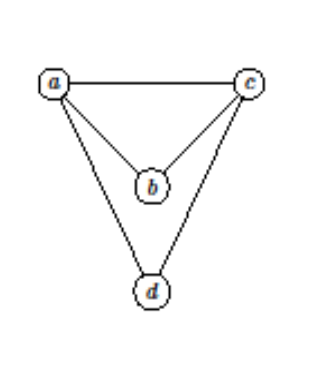
\includegraphics[scale=0.65]{grafo1}
\end{center}

Un mismo grafo puede tener distintas representaciones, pero representar la misma información. En ese caso, decimos que son isomorfos.
\begin{center}
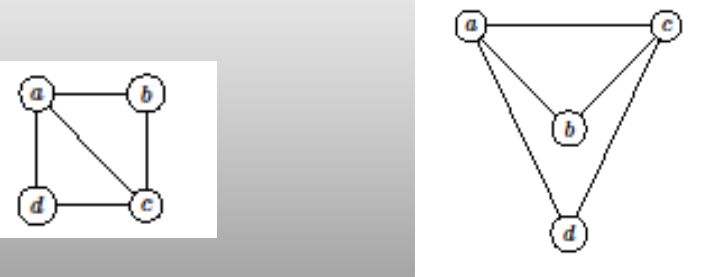
\includegraphics[scale=0.65]{isomorfia grafos}
\end{center}

Es fácil destacar que para referirnos a una arista en este tipo de grados es indiferente el orden en el que nombre los vértices que conecta puesto que al tratarse de un grafo no dirigido, hemos definido cada arista como un subconjunto de cardinal dos, así pues $\{v_i,v_j\}=\{v_j,v_i\}$.

\subsubsection*{Pseudografos}
Cumplen la definición ordinaria que se ha dado de grafo, a excepción de que en este caso se permiten las \textbf{autoaristas}, es decir, que suprimimos la condición de que $v_i\neq v_j$ para la autoarista $e=\{v_i,v_j\}$.

\begin{center}
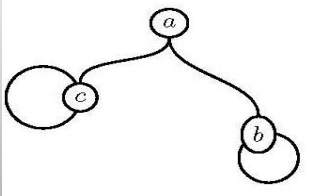
\includegraphics[scale=0.65]{pseudografo}
\end{center}

A estas aristas se las conoce como lazos o bucles.

\subsubsection*{Multigrafos}
Reúnen todas las condiciones anteriores, con la única excepción de que entre dos vértices puede haber más de una arista.

\begin{center}
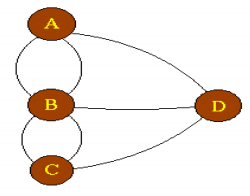
\includegraphics[scale=0.65]{multigrafo}
\end{center}

Es decir, a pesar de que las aristas unen mismos vértices hay que llamarlas de forma distinta porque representan caminos distintos entre ambos puntos.

\subsubsection*{Grafo dirigido}
Los grafos dirigidos reúnen las mismas características y peculiaridades de los grafos no dirigidos, a excepción de que en este caso las aristas poseen dirección y pasan a llamarse \textbf{arcos}. Con lo cual podemos decir que poseen los siguientes elementos:
\begin{itemize}
\item Conjunto de vértices: $V=\{v_1, ..., v_n\}$

\item Conjunto de arcos: $A=\{(v_i,v_j), ...\}$

	Es decir, en este caso los arcos representan la relación de adyacencia entre dos vértices. Cuando $uAv$ decimos que el arco está orientado desde el origen $u$ hasta el destino $v$ y que el destino $v$ es adyacente al origen $u$. Como relación que es, ahora en vez de ser subcojuntos de $V$ son \textbf{pares} de $V$.
\end{itemize}

\begin{center}
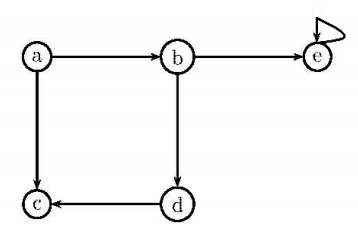
\includegraphics[scale=0.65]{grafo dirigido}
\end{center}

\subsection*{\underline{Grado de un vértice: adyacencia}}
Decimos que dos vértices son adyacentes o vecinos si existe una arista que los une. En ese caso los vértices son los extremos\footnote{Si $v$ es extremo de la arista $a$ se dice que $a$ incide en él} de la arista.
$$uAv\Leftrightarrow\exists a=\{u,v\}\in E$$

El \textbf{grado de un vértice} es el número de aristas\footnote{En los pseudografos, las autoaristas cuentan dos veces como arista incidente} que inciden sobre él. Cuando un vértice posee grado 0 se le llama aislado y en los \textbf{GRAFOS NO DIRIGIDOS} el grado es sinónimo del número de vértices adyacentes.

En los grafos dirigidos, distinguimos entre \textbf{grado de entrada} ($gr^-(v)$): número de aristas de las que es origen el vértice y \textbf{grado de salida}($gr^+(v)$): número de aristas de las que es destino.

\begin{center}
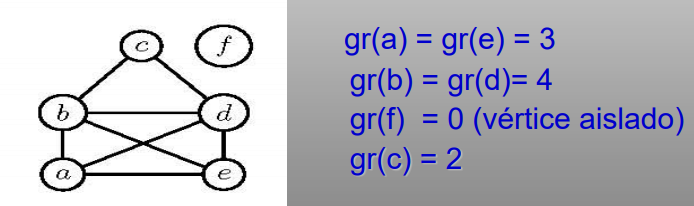
\includegraphics[scale=0.65]{adyacencia}
\end{center}

\subsubsection*{Teorema de los apretones de manos}
Sea $G$ un grafo, entonces se tiene que el sumatorio de los grados es el doble del número de aristas:
$$\sum_{v\in V} gr(v)=2|E|$$
\underline{Demostración}:

La demostración es sencilla, puesto que si una arista conecta dos vértices y el grado de un vértice es el número de aristas que inciden sobre él, se tiene que al sumar los grados de cada vértices, las aristas que unen dos se cuentan dos veces.

\underline{\textbf{Corolario}}:

Es evidente de forma inmediata que cualquier grafo dirigido tiene un número par de vértices de grado impar.

\subsubsection*{Teorema}
El mismo teorema pero para grafos dirigidos nos dice que:
$$\sum_{v\in V}gr^+(v)+\sum_{v\in V}gr^-{v}=|A|$$

Que se ve de forma evidente que entendiendo la demostración del anterior, este es cierto.

\subsubsection*{Grafo completo y regular}
Para un número de vértices mayor que 1, se dice que un \textbf{grafo es completo de orden $n$} si cada par de vértices escogidos son adyacentes.

\begin{center}
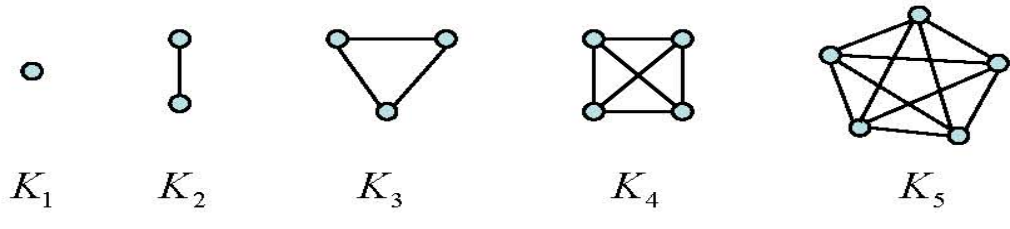
\includegraphics[scale=0.65]{grafo completo}
\end{center}

Se llama \textbf{grafo regular de grado }$K\geq 0$ o grafo $K-$regular a los grafos cuyos vértices poseen todos grado $K$.

\begin{center}
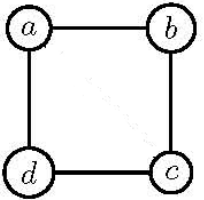
\includegraphics[scale=0.65]{grafo regular}
\end{center}


\subsubsection*{Matriz de Adyacencia}
Para representar las relaciones que existen en un grafo entre los distintos vértices del mismo se puede utilizar lo que denominamos \textbf{matriz de adyacencia}.

\begin{center}
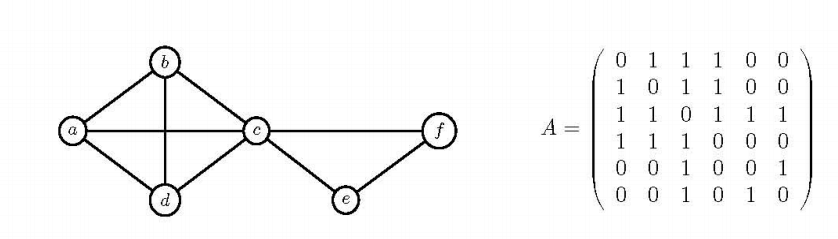
\includegraphics[scale=0.65]{matriz de adyacencia}
\end{center}

En esta matriz, las filas y las columnas son los vértices (en el mismo orden) y un uno en cierta coordenada significa que los vértices columna y fila están relacionados por medio de una arista.

Es fácil observar que las matrices en \textbf{grados no dirigidos} serán simétricas y su diagonal será 0 (si no se permiten los pseudografos). No ocurre esto con los grafos dirigidos, en los que por convenio se tiene que las filas representan los vértices origen y las columnas los vértices destino, por lo que ya no se guarda esta relación de simetría entre ambos.

\begin{center}
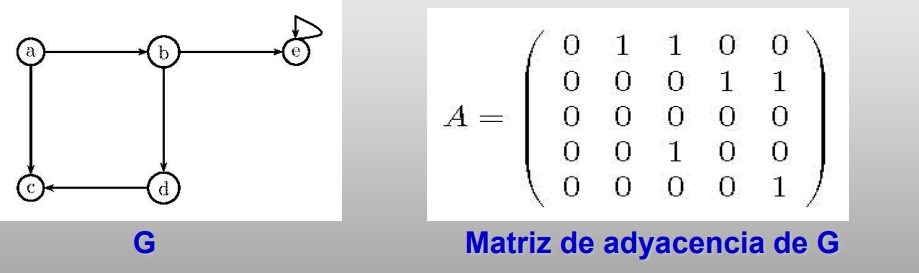
\includegraphics[scale=0.65]{matriz grafo dirigido}
\end{center}

\subsubsection*{Tabla de adyacencia}

\begin{center}
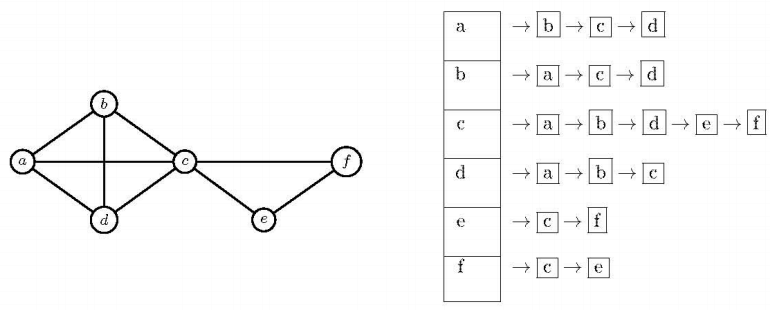
\includegraphics[scale=0.65]{tabla de adyacencia}
\end{center}

\subsubsection*{Subgrafos}
Dado un grafo $G=(V,E)$ y otro $G`=(V',E')$ se dice que $G'$ es un subgrafo de $G$ si $V'\subset V$ y $E'\subset E$, es decir, si es un subconjunto del grafo principal.

\begin{center}
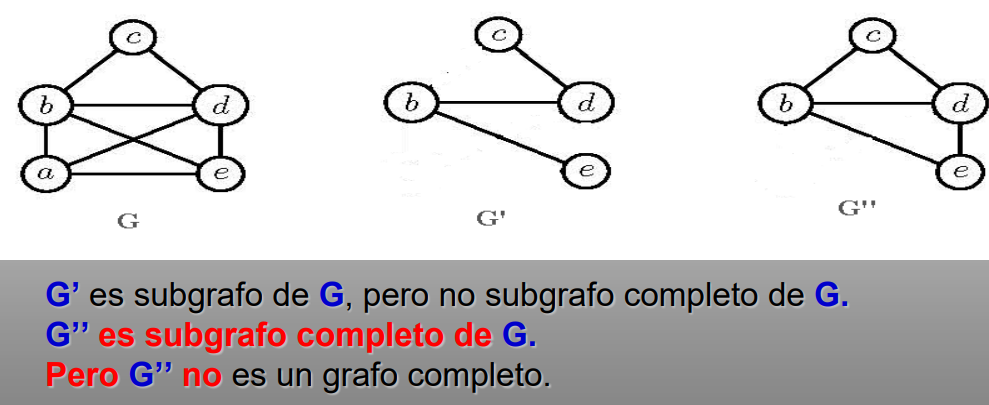
\includegraphics[scale=0.65]{subgrafos}
\end{center}

Además se llama subgrafo completo si el subgrafo posee todas las aristas que conectan los vértices del subgrafo en el grafo principal.

\section*{CAMINOS Y CONECTIVIDAD}
\subsection*{\underline{Movimientos por el grafo}}
\subsubsection*{Recorridos y circuitos}
Un \textbf{recorrido}\footnote{Los conceptos explicados en este apartado son aplicables a los grafos dirigidos teniendo en cuenta que las aristas ahora poseen dirección} es una sucesión de vértices del grafo que \textbf{permite la repetición de vértices y aristas}:
$$R=\{v_0,..., v_n\}: \{v_i, v_{i+1}\}\in E$$
Decimos entonces que el recorrido conecta el vértice inicial con el final, que su longitud es $n$ y cabe destacar que aunque el recorrido vaya por el mismo ``sendero'' no es lo mismo ir de $c$ a $e$ que al revés, es decir, son recorridos distintos.

\begin{center}
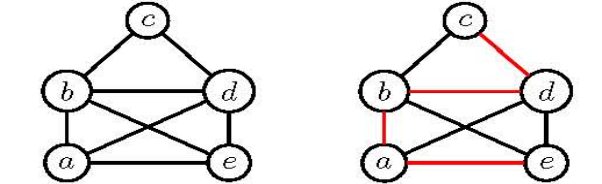
\includegraphics[scale=0.65]{recorridos}
\end{center}

Por otro lado, cuando un \textbf{recorrido comienza y termina en el mismo sitio} se le llama \textbf{circuito}.

\subsubsection*{Caminos y ciclos}
Un \textbf{camino} es un recorrido que no permite repetir ni vértices ni aristas (salvo el primero y el último):
$$C=\{v_0, ..., v_n\}: v_i\neq v_j: \forall 0< i < j< n$$
Cuando un \textbf{camino comienza y termina en el mismo vértice}se le conoce como \textbf{ciclo}.

\begin{center}
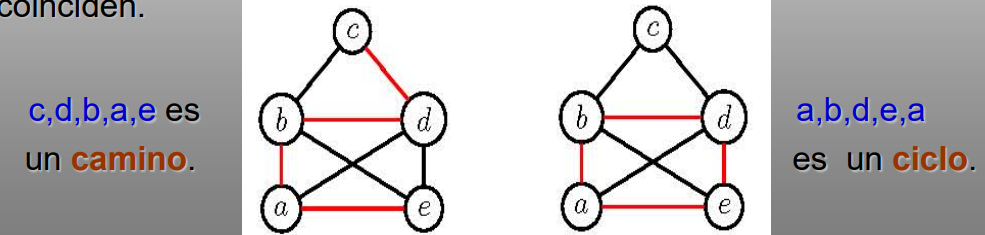
\includegraphics[scale=0.65]{camino y ciclo}
\end{center}

\underline{\textbf{Teorema}}: de cualquier recorrido se puede extraer un camino:
$$\forall x,y\in V: \exists R=\{x, ..., y\}\Leftrightarrow \exists C=\{x,..., y\}$$
\underline{Demostración}:

Si directamente tenemos el camino ya hemos acabado, en caso contrario lo que ocurre es que hay vértices se repiten más de una vez, con lo cual podemos simplificar el problema al siguiente dibujo:
\begin{center}
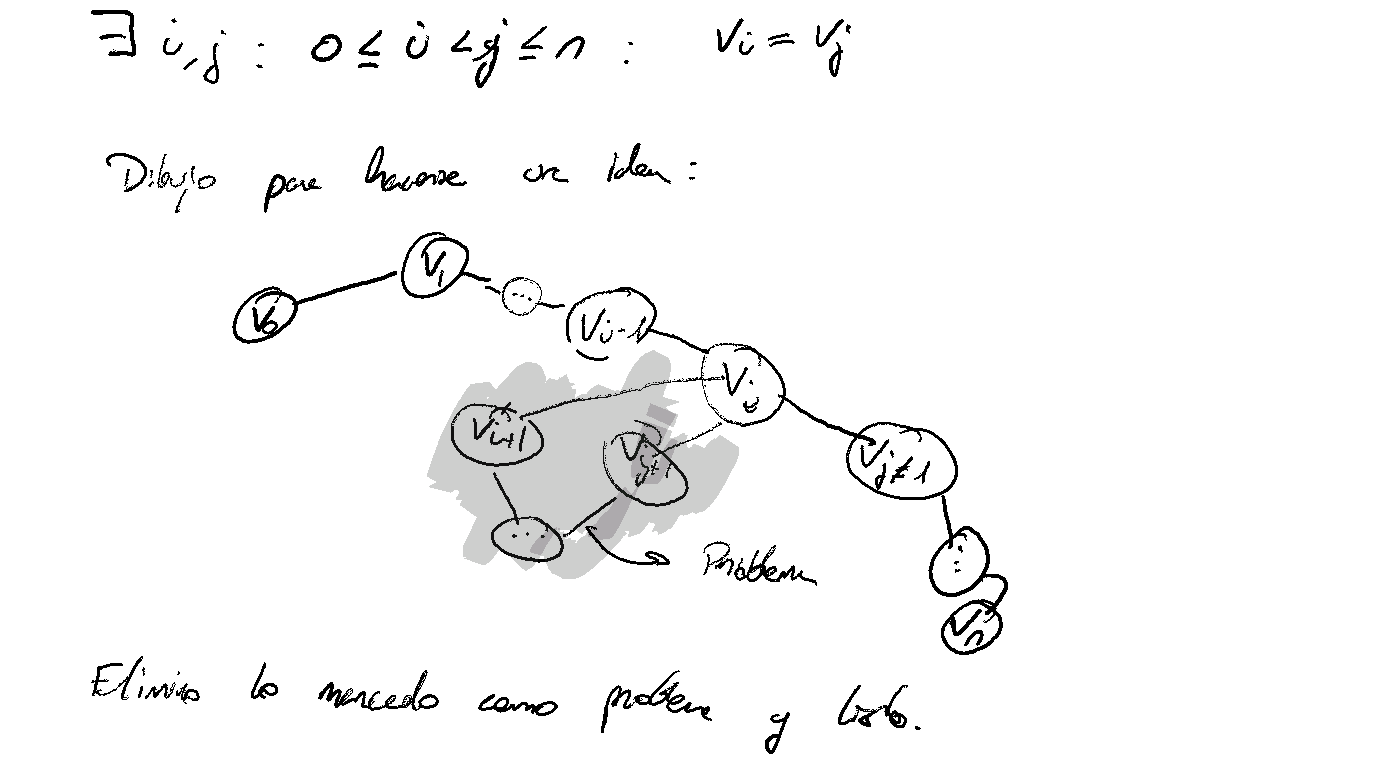
\includegraphics[scale=0.65]{teorema camino}
\end{center}
La implicación de derecha a izquierda es trivial por la propia definición de camino, para la otra implicación la idea es que se puedan ``cortar'' esos flecos del dibujo para poder extraer el recorrido limpio.



\subsection*{\underline{Grafo Conexo}}
Si definimos la relación $C\subset V^2$, en un grafo no dirigido, de manera que dos vértices están conectados si y sólo si existe un camino entre ambos, esto define una relación de equivalencia\footnote{En general en los grafos dirigidos no forma una relación de equivalencia} en $V$:
\begin{itemize}
\item Reflexiva:
$$aCa\Leftrightarrow C=\{\emptyset\}$$

\item Simétrica:
$$aCb\Rightarrow C_1=\{a, ..., b\}\Rightarrow C_2=\{b, ..., a\}\Rightarrow bCa$$

\item Transitividad:
$$\begin{cases}xCy\Rightarrow \exists C_1=\{x, ..., y\}\\\ yCz\Rightarrow C_2=\{y, ..., z\} \end{cases} \Rightarrow \exists R=\{x, ..., y, ..., z\}\stackrel{Teorema}{\Rightarrow} \exists C=\{x,..., y, ..., z\} $$
\end{itemize}

\begin{center}
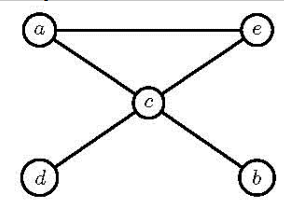
\includegraphics[scale=0.80]{grafo conexo}
\end{center}

Decimos entonces que un \textbf{grafo es conexo} si y solo si para cada par de vértices del grafo siempre existe un \textbf{camino entre ambos}, es decir, que el conjunto cociente tiene sólo un elemento. Una buena forma de demostrar esta propiedad en un grafo es construir un recorrido que pase por todos los vértices y por el teorema de la parte de caminos, siempre podremos extraer un camino entre dos vértices.

\underline{\textbf{Proposición}}:

Una consecuencia es que si un grafo es conexo entonces si tiene $n$ vértices tiene como mínimo $n-1$ aristas.
 
\subsubsection*{Componentes conexas, puntos de corte y aristas puente}
\underline{\textbf{Componentes conexas}}:

Cada clase de equivalencia del conjunto cociente definido se denomina \textbf{componente conexa}, es decir, son los mayores subgrafos conexos del grafo principal.

\begin{center}
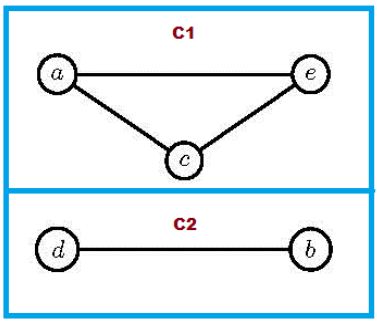
\includegraphics[scale=0.65]{componentes conexas}
\end{center}

Si el grafo es conexo solo existe una clase de equivalencia y en consecuencia una componente conexa, pero si no lo es entonces existirán más componentes conexas\footnote{A los vértices aislados se les llama componentes conexas triviales}.

\underline{\textbf{Puntos de corte}}:

Denominamos puntos de corte a aquellos puntos que tras ser eliminados junto con las aristas que inciden en él, divide al grafo en más componentes conexas.
\begin{center}
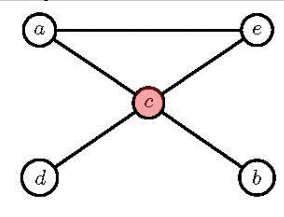
\includegraphics[scale=0.55]{punto de corte}
\end{center}

\underline{\textbf{Aristas puentes}}

Definimos las aristas puente como las aristas que si se eliminan descomponen el grafo en más componentes conexas, o dicho de otra manera, en dos subgrafos no conectados entre ellos.

\begin{center}
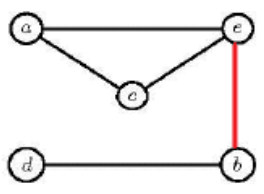
\includegraphics[scale=0.65]{arista puente}
\end{center}

\subsubsection*{Lemas de caracterización}
En un grafo conexo, $v\in V$ es un \textbf{punto de corte} si existen dos puntos para los que cualquier camino que escoja y que conecte a ambos contiene necesariamente al punto de corte:
$$\exists x, y \in V: \forall C=\{x, ..., y\}: v\in C$$

En un grafo conexo, $e\in E$ es una \textbf{arista puente} si y sólo si no se encuentra contenida en ningún ciclo posible del grafo.

\subsection*{\underline{Grafos eurelianos}}
Cuando un circuito pasa por todas las aristas de un grafo sin repetir ninguna se lo conoce como \textbf{circuito eureliano}. A los grafos que los contienen se los denomina \textbf{grafos eurelianos}.

\begin{center}
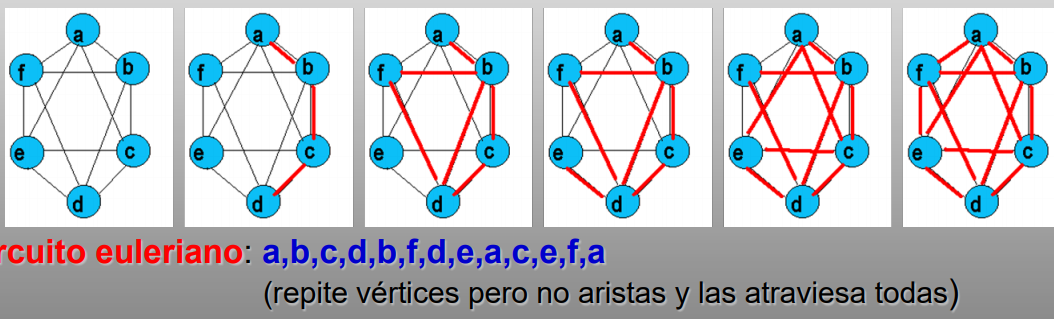
\includegraphics[scale=0.55]{grafo eureliano}
\end{center}

Cuando lo que se consigue no es un circuito sino un recorrido eureliano se dice que el grafo es un \textbf{grafo semieureliano} y es condición excluyente de ser eureliano, es decir, o se es eureliano o se es semieureliano pero uno no es un caso particular del otro.

\subsubsection*{Teorema de Euler}
Un grafo es eureliano si y solo si es conexo y todos su vértices son de grado par:
$$eureliano \Leftrightarrow \mbox{conexo }\wedge \forall v\in V: gr(v)=2k: k\in \mathbb N$$
Un grafo es semieureliano si y solo si es conexo y todos sus vértices son de grado par salvo únicamente dos de grado impar:
$$semieureliano \Leftrightarrow \mbox{conexo }\wedge \forall v\in V\mbox{\textbackslash}\{v_i, v_j\}: gr(v)=2k: gr(v_i)\neq 2k \neq gr(v_j)$$

\underline{Demostración}:

Se pueden usar métodos algebraicos pero en el fondo es liar la demostración. Si pensamos que este tipo de circuitos no pueden repetir aristas, cada vez que entramos por una arista en un vértice tiene que existir otra por la que se pueda salir para no usar por la que se ha venido, es decir, que el grado de todos los vértices tiene que ser par. En caso de que solo halla dos vértices que sean de grado impar, quiere decir que en uno de ellos se comienza y en el otro se termina pues esa arista de más es para empezar el recorrido o para terminarlo.

\subsubsection*{Búsqueda de circuitos eurelianos}
Aunque la caracterización de un grafo eureliano es simple, la búsqueda de dicho recorrido puede ser tediosa, por lo que se presenta el siguiente algoritmo:
\begin{enumerate}
\item Escogemos un circuito cualquiera
\item Borramos las aristas de ese circuito del grafo y nos queda otro subgrafo que estará dividido en varias componentes conexas.
\item Dentro de estas componentes buscamos circuitos eurelianos y si son muy complejas lo tratamos como si fuese otro grafo volviendo al punto 1
\item Cuando hemos encontrado los pequeños circuitos eurelianos en cada componente y solo se usan las aristas de esa componente, podemos ``pinchar'' esos circuitos en el circuito del inicio sin que haya ningún problema.
\end{enumerate}
\begin{center}
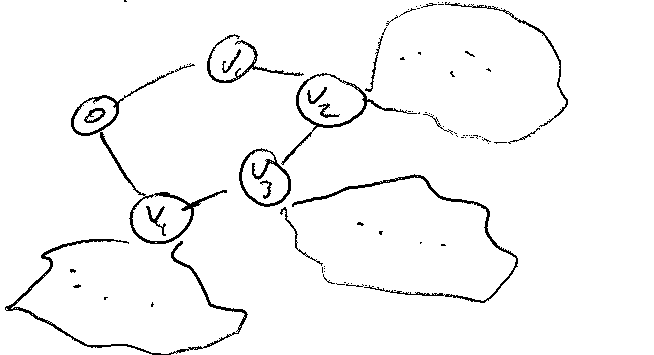
\includegraphics[scale=0.65]{algoritmo de euler}
\end{center}

\subsection*{\underline{Grafos Hamiltonianos}}
Cuando un ciclo pasa por todos los vértices de un grafo sin repetir ninguno se lo conoce como \textbf{ciclo hamiltoniano}. A los grafos que los contienen se los denomina \textbf{grafos hamiltonianos}.
\begin{center}
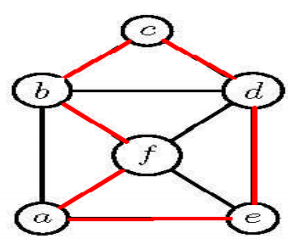
\includegraphics[scale=0.75]{grafo hamiltoniano}
\end{center}

\subsubsection*{Condiciones necesarias y suficientes}
Sin embargo, para este problema no se conoce ningún teorema que caracterice a este tipo de grafos como ocurre con los eurelianos. Pero si que existen una serie de condiciones que son necesarias o suficientes para poder descartar casos.

\underline{\textbf{Condiciones necesarias}}
\begin{itemize}
\item Conexo.
\item No puede tener vértices de grado 1. Si tiene más de un vértice, todos sus vértices son de grado $\geq 2$.
\item No puede tener puntos de corte.
\item No puede tener aristas puente.
\end{itemize}

\underline{\textbf{Condiciones suficientes}}
\begin{itemize}
\item Teorema de Dirac:
$$|V|\geq 3: \forall v\in V: gr(v)\geq \frac{n}{2}\Rightarrow HAMILTONIANO$$

\item Teorema de Ore:
$$|V|\geq 3: \forall u,v\in V: \nexists e=\{u,v\}\in E: gr(u)+gr(v)\geq n\Rightarrow HAMILTONIANO$$
\end{itemize}

\subsection*{\underline{Isomorfismo de grafos}}
Decimos que dos grafos son isomorfos cuando existe una función biyectiva entre los vértices que preserve la adyacencia.

\begin{center}
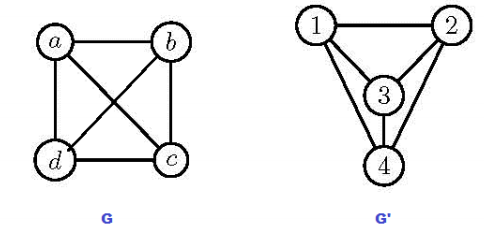
\includegraphics[scale=0.65]{Isomorfismo de grafos}
\end{center}

Es decir, que si tirásemos de los vértices, como si se hubiesen liado las aristas, hasta colocar los vértices de la misma forma resultaría que salvo los nombres ambos serían el mismo grafo.

\subsubsection*{Condiciones necesarias}
Lamentablemente, no existe ningún teorema que caracterice a estos grafos por lo que solo basta con conformarse con una serie de condiciones que descartan casos que comprobar:
\begin{itemize}
\item Mismo número de vértices.
\item Mismo número de aristas.
\item Mismo número de vértices con un mismo grado $n$.
\item Si uno de los grafos tiene como subgrafo a $K_n$ (salvo renombramiento de vértices), lo mismo debe suceder en el otro grafo.
\item Si uno de los grafos es euleriano o hamiltoniano o conexo el otro también ha de serlo.
\item Si en uno de los grafos hay un ciclo de longitud $n$, lo mismo debe suceder en el otro grafo.
\item En general, no diferir en alguna propiedad que preservan las biyecciones que preservan la adyacencia.
\end{itemize}

\subsection*{\underline{Árboles}}
Un árbol es un grafo no dirigido y conexo sin ciclos no triviales (que no sean de longitud 0). Cuando destacamos un vértice sobre los demás, llamamos a este raíz.

\begin{center}
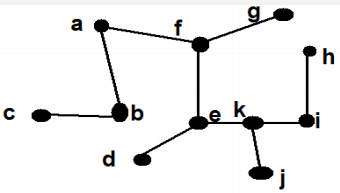
\includegraphics[scale=0.65]{arbol}
\end{center}

\subsubsection*{Propiedades}
Cualquier árbol tal y como lo hemos definido cumple las siguientes propiedades:
\begin{itemize}
\item Entre cada par de vértices de T hay un camino único
\item Toda arista de T es una arista puente. Al eliminar 
cualquier arista de T se desconecta el árbol es dos 
componentes conexas que son a su vez árboles.
\item $|E| = |V| - 1$
\end{itemize}

Además si un árbol tiene raíz podemos distinguir en él las siguientes partes:
\begin{itemize}
\item A los vértices se les llaman habitualmente \textbf{nodos}. 
\item El \textbf{nivel} de un nodo es la longitud del camino desde la raíz del árbol a dicho nodo. Por tanto el nivel de la raíz es 0.
\item Se llaman \textbf{hijos} de un nodo $x$ de nivel $i$ a los nodos de nivel $i + 1$ adyacentes a x.
\item Todo nodo es \textbf{padre de sus hijos}.
\item Los hijos de un mismo padre son \textbf{hermanos}.
\item La raíz es el único nodo que no tiene padre.
\item Se llaman \textbf{hojas a los nodos sin hijos}. Se llaman \textbf{nodos internos} a los demás.
\item Las \textbf{ramas} del árbol son los caminos desde su raíz a las hojas.
\item La \textbf{altura (o talla)} del árbol es la longitud de su rama más larga.
\end{itemize}

\chapter*{COMBINATORIA}
En este tema vamos a estudiar la combinatorio, entre cuyas aplicaciones está el determinar de forma precisa el cardinal de un conjunto determinado. Por lo que consiste básicamente en métodos de conteos de distintas cosas.

\section*{MÉTODOS DE CONTEO}
\subsection*{\underline{Principios elementales del conteo}}
El método general para el recuento concreto de casos será:
\begin{itemize}
\item Definir un conjunto $S$ que contendrá a todas las posibilidades.
\item Calcular $|S|$ utilizando los métodos de conteo.
\end{itemize}

Para realizar estas labores de cuantificación, podemos tener en cuenta las siguientes reglas aplicadas para conjuntos FINITOS:
\begin{itemize}
\item \textbf{Inclusión}:
$$S\subset A\Rightarrow |S|\leq |A|$$
\item \textbf{Principio de inclusión-exclusión}
$$|A\cup B|=|A|+|B|-|A\cap B|$$
\item \textbf{Exclusión}:
$$|A\mbox{\textbackslash}B|=|A|-|A\cap B|$$
\item \textbf{Regla del Producto}:
$$|A\times B| = |A|\cdot |B|$$
\item \textbf{Asignaciones posibles}:
$$|(A\rightarrow B)|=|B|^{|A|}$$
\item \textbf{Biyección}:
$$\exists f: A\rightarrow B \mbox{ biyectiva}\Rightarrow |A|=|B|$$
\item \textbf{Conjunto de Partes}:
$$|P(A)|=2^{|A|}$$
\end{itemize}

\subsubsection*{Recuento por filas y columnas}
En ocasiones, será conveniente representar el conjunto del que queremos hallar el cardinal como una relación binaria sobre dos subconjuntos del mismo, es decir, $R\subset X\times Y$. Definimos ahora:
$$x_0\in X: y_0\in Y\Rightarrow \begin{cases}F_{x_0} = R\cap (\{x_0\}\times Y) \\ C_{y_0} = R\cap (X\times \{y_0\})\end{cases}$$
Es decir\footnote{De forma gráfica se puede ver como el número de puntos que hay (pares) en la vertical de un punto del eje $x$}, para cada coordenada de la fila definimos el conjunto $F_{x_0}$ que representa el número de pares que tienen a $x_0$ por primera coordenada y de forma análoga con $y_0$ y $C_{y_0}$.

Ahora si llamamos $\mathbb R= \{R: R\subset X\times Y\}$ al conjunto de todas las posibles relaciones binarias de ese conjunto, las aplicaciones:
$$\begin{cases}f_{x_0}: \mathbb R\rightarrow \mathbb N &\mbox{ donde }f_{x_0}(R)= |F_{x_0}(R)| \\ c_{y_0}: \mathbb R\rightarrow \mathbb N &\mbox{ donde }c_{y_0}(R)= |C_{y_0}(R)| \end{cases}$$
Asignan a cada relación binaria y a cada elemento de cada conjunto, el cardinal de su fila o de su columna respectivamente (es decir, es lo mismo que lo explicado arriba pero asignando el valor en función de la relación definida).

De este modo es trivial que:
$$|R|=\sum_{x_0\in X}f_{x_0}(R)=\sum_{y_0\in Y}c_{y_0}(R)$$
Y a modo de corolario, si $\forall x_0\in X: f_{x_0}(R)=\lambda$ y $\forall y_0\in Y: c_{y_0}(R)=\varphi$, entonces:
$$|R|=\lambda |X|=\varphi |Y|$$

\section*{CÁLCULO DE AGRUPACIONES}
\subsection*{\underline{Variaciones, combinaciones, permutaciones...}}
Cuando escogiendo elementos de un conjunto hacemos grupos en determinadas condiciones, surge la pregunta de: ¿Cuántos grupos distintos podré formar? Para poder responder adecuadamente esta pregunta hace falta tener en cuenta las condiciones en las que se forman esos grupos y qué se considera distinto en cada caso.

\subsubsection*{Variaciones sin repetición}
Llamamos \textbf{variaciones sin repetición} de $n$ elementos tomados de $m$ en $m$ y lo denotamos por $V_m^n$ a los distintos grupos que se pueden hacer  SIN REPETIR LOS ELEMENTOS DEL CONJUNTO A REPARTIR, tomándolos de $m$ en $m$ y teniendo en cuenta que para mismos elementos en un grupo pero órdenes distintos, las asociaciones son distintas, es decir, $abc\neq bca$ aunque posean los mismos elementos.

Para dar respuesta a este problema, nos preguntamos cuál es el cardinal del conjunto de las funciones inyectivas que van de un conjunto $|N|=n$ a otro $|M|=m$:
$$V_m^n=|m\hookrightarrow n|=\prod_{i=1}^m (n-i+1)=\frac{n!}{(n-m)!}$$
Por convenio tenemos que $n<m\Rightarrow V_m^n=0$ y que $m=0\Rightarrow V_m^n=1$.

\subsubsection*{Permutaciones sin repetición}
Las \textbf{permutaciones sin repetición} son un caso concreto de las variaciones sin repetición donde $m=n$, es decir, la única diferencia es en qué orden se encuentran los elementos puesto que todos los conjuntos poseen a todos los posibles elementos. En este caso y aplicando la fórmula de antes:
$$V_n^n=\frac{n!}{(n-n)!}=n!$$

\subsubsection*{Variaciones con repetición}
Llamamos \textbf{variaciones con repetición} de $n$ elementos tomados de $m$ en $m$ y lo denotaremos por $VR_m^n$ a los distintos grupos que podemos formar agrupando $n$ elementos de $m$ en $m$ PUDIENDO SELECCIONAR EL MISMO ELEMENTOS MÁS DE UNA VEZ pero distinguiendo agrupaciones distintas para órdenes distintos.

En este caso la pregunta es ¿cuántas funciones totales hay de un conjunto $|N|=n$ a otro $|M|=m$?
$$VR_m^n|=(m\hookrightarrow n)|= n^m$$

\subsubsection*{Combinaciones sin repetición}
Las combinaciones son variaciones en las que no importa el orden de los elementos escogidos, es decir, nos preguntamos por el número de subconjuntos del conjunto de índices a escoger cuyo cardinal es el especificado. Concretamente, las \textbf{combinaciones sin repetición} son aquellas en las que NO SE PUEDE ESCOGER AL MISMO INDIVIDUO MÁS DE UNA VEZ Y SE DEBEN FORMAR GRUPOS DEL CARDINAL ESPECIFICADO.
$$\binom{n}{m}=\frac{n!}{m!(n-m)!}$$
\underline{\textbf{Propiedades}}:
\begin{enumerate}
\item $\forall n,m \in \mathbb N : n<m\Rightarrow \binom{n}{m} = 0$
\item $\forall n \geq 0: \binom{n}{0} = \binom{n}{n} = 1$
\item $\forall n\geq 0 : \binom{n}{1}= n$
\item $\forall n,m\in \mathbb N: \binom{n}{m} = \binom{n}{n-m}$
\item $\forall n,m\in \mathbb N: \binom{n-1}{m-1} +\binom{n-1}{m}$
\item $\sum_{m = 0}^{n}\binom{n}{m} = 2^n$
\item $\sum_{m = 0}^{n}(-1)^m\binom{n}{m} = 0$
\end{enumerate}

\subsubsection*{Combinaciones con repetición}
De nuevo, hablamos de variaciones en las que no importa el orden de los elementos escogido, pero con la novedad de que en las \textbf{combinaciones con repetición} SE PUEDE ESCOGER EL MISMO INDIVIDUO MÁS DE UNA VEZ. 
$$\begin{bmatrix} n \\ m\end{bmatrix} = \binom{n+m-1}{m}$$
\underline{Demostración}:

La demostración de dicho resultado es porque podemos considerar cada posible combinación como una palabra binaria (formada por 0 y 1) de la siguiente forma:
$$\overbrace{111\cdots 1}^{k_1} \ 0 \ \overbrace{11\cdots 1}^{k_2} \ 0 \cdots 0 \ \overbrace{11\cdots 1}^{k_n}$$
Donde cada $k_i$ es el número de veces que se repite cada elemento y cada $0$ es un separador de elementos; los 1 corresponden al elemento que se repite $k_i$ veces. De este modo, el problema queda reducido al cálculo del número de palabras binarias de longitud $n+m-1$ porque tenemos $m$ elementos útiles y $n-1$ separadores.

\subsubsection*{Teorema Binomial}
Más conocido como el binomio de Newton afirma que:
$$\forall n \in \mathbb N: (a+b)^n = \sum_{i = 0}^{n} \binom{n}{i} a^{n-i}b^i$$
Es decir, que podemos calcular la potencia enésima de cualquier suma gracias a esta fórmula. La demostración es sencilla por inducción.

\subsubsection*{Principio de Inclusión-Exclusión}
A pesar de que se ha visto la forma simplificada para 2 conjuntos anteriormente, este es una generalización para $n$ conjuntos:

Sean $A_0, A_1, \ldots, A_{n-1}$ conjuntos finitos, podemos definir $\alpha_i$ como la suma de los cardinales de todas las intersecciones de $i$ conjuntos de los $n$ que hay, es decir:
$$\alpha_i = \sum_{I\subseteq n: |I|=i} | \bigcap_{j\in I} A_j|$$
De este modo, para calcular el cardinal de la unión de todos los conjuntos basta con atenerse a:
$$|\bigcup_{i=1}^{n} A_i| = \sum_{i = 1}^{n} (-1)^{i-1}\alpha_i$$
Es decir, que tenemos que sumar o restar las sucesivas intersecciones 2 a 2, 3 a 3, 4 a 4, etc. al total.


\subsubsection*{Teorema Multinomial}

\subsubsection*{Repartos ponderados}
Dados $X=\{a_1, a_2, \cdots, a_n\}$ y $k\in \mathbb N\setminus\{0\}$ se define el reparto ponderado como el reparto de los $n$ elementos del conjunto $X$ en $k$ subconjuntos $C_i\subseteq X: |C_i| = m_i,\ 1\leq i \leq k$ de forma que la suma de los cardinales de todos sea el cardinal total, es decir, $\sum_{i=1}^k m_i =n$.

\subsubsection*{Permutaciones circulares}

\chapter*{LÓGICA PROPOSICIONAL}
\section*{DEFINICIÓN Y LENGUAJE DE LA LÓGICA}
La lógica estudia la fundamentación del concepto de certeza y todo lo que esta involucra, además estudia las reglas del pensamiento y de la argumentación válida para poder discernir cuando es o no un pensamiento correcto y cuando es cierta la deducción de unas conclusiones a partir de ciertas premisas.

\subsection*{\underline{Sintaxis de la lógica proposicional}}
\subsubsection*{Alfabeto de la lógica proposicional}
En primer lugar, hemos de hacer una distinción entre el lenguaje natural (que admite ambigüedades) y el lenguaje de la lógica (que no las admite) por lo que será necesario disponer de una serie de símbolos que no dejen espacio a la interpretación, es decir, nuestro lenguaje va a estar formado por:
\begin{itemize}
\item \underline{\textbf{Símbolos lógicos}}: $\{\bot, \top, \neg, \wedge, \vee, \rightarrow, \leftrightarrow \}$
	\begin{itemize}
	\item \textbf{Constantes lógicas}: $\{\bot, \top\}$: Indican la falsedad o veracidad respectivamente.
	
	\item \textbf{Conectivas unarias}: $\{\neg\}$: Define la relación de negación vista en el apartado de lógica elemental visto en este libro.
	
	\item \textbf{Conectivas binarias}: $\{\wedge, \vee, \rightarrow, \leftrightarrow\}$:	Definen las relaciones de ``y'', ``o'', implicación y equivalencia vistas en el apartado de lógica elemental de este libro.
	\end{itemize}
\item \underline{\textbf{Símbolos auxiliares}}: $\{(,)\}$

Son símbolos que denotan la precedencia de operaciones

\item \underline{\textbf{Signatura}}: $\{\Sigma\}$

Denota al conjunto de símbolos de proposición. La base del estudio de la lógica proposicional son las \textbf{proposiciones}. Estas son oraciones declarativas que o bien es cierta o bien es falsa, pero que no admite ambigüedades. Dentro de las proposiciones podemos distinguir:
	\begin{itemize}
	\item \textbf{Proposiciones atómicas}:

	Las denotamos por letras minúsculas y no se pueden descomponer en otras 	más simples, p. ej., $p =$``Mario compró un coche'' es una proposición 	atómica.

	\item \textbf{Proposiciones compuestas}:

	Estas proposiciones son las que están formadas por proposiciones atómicas y por las relaciones que podamos establecer entre ellas a través de conectivas lógicas.
	\end{itemize}
\end{itemize}

Con lo cual, definimos el alfabeto sobre el que vamos a trabajar como:
$$A_\Sigma = \Sigma\cup \{\bot, \top, \neg, \wedge, \vee, \rightarrow, \leftrightarrow\}\cup \{(,)\}$$
De modo análogo, definimos el conjunto de todas las posibles palabras que podemos formar sobre este alfabeto como:
$$A_\Sigma^*$$

\subsubsection*{Lenguaje de la lógica proposicional}
Sin embargo, no todas las palabras que formemos sobre el alfabeto definido como $A_\Sigma$ tienen sentido. Como sabemos que lo único que tiene algún sentido y está bien construido son las proposiciones atómicas, hay que definir de alguna forma unas \textbf{reglas de formación} que permitan determinar qué palabras tienen sentido, a las que llamaremos fórmulas:
\begin{itemize}
\item Las proposiciones atómicas y las constantes lógicas son fórmulas.
\item Si $\varphi$ es una fórmula, entonces $\neq \varphi$ es una fórmula
\item Si $\varphi_1$ y $\varphi_2$ son fórmulas, entonces $\varphi_1 \wedge \varphi_2$ es una fórmula.
\item \item Si $\varphi_1$ y $\varphi_2$ son fórmulas, entonces $\varphi_1 \vee \varphi_2$ es una fórmula.
\item Si $\varphi_1$ y $\varphi_2$ son fórmulas, entonces $\varphi_1 \rightarrow \varphi_2$ es una fórmula.
\item Si $\varphi_1$ y $\varphi_2$ son fórmulas, entonces $\varphi_1 \leftrightarrow \varphi_2$ es una fórmula.
\end{itemize}
De este modo, dada una signatura $\Sigma$ concreta, queda determinado por completo el lenguaje válido con el que vamos a trabajar y que vamos a denotar por $L_\Sigma$: el conjunto de todas las fórmulas con signatura $\Sigma$. A estas fórmulas válidas las denotamos por letras griegas usualmente $\varphi, \psi, \xi, ...$.

\subsubsection*{Principio de Inducción Estructural}
Dada una propiedad P concreta, la demostración de que esa propiedad se atiene a todas las fórmulas definidas en nuestro lenguaje de la lógica es correcta si verificamos:
\begin{itemize}
\item \textbf{Caso base}

Toda fórmula atómica tiene la propiedad P

\item \textbf{Pasos inductivos}
	\begin{itemize}
	\item \textbf{Negación ($\neg \varphi$)}: sabiendo que la fórmula $\varphi$ posee la propiedad $P$, demostrar que $\neg \varphi$ también tiene dicha propiedad.
	
	\item \textbf{Conectiva ($\varphi_1 \square \varphi_2$)}: sabiendo que $\varphi_1$ y $\varphi_2$ la poseen, demostrar que $\varphi = \varphi_1 \square \varphi_2$ la posee también.
	\end{itemize}
\end{itemize}

\subsubsection*{Principio de Unicidad Estructural}
Podemos determinar de modo único el proceso de construcción que ha seguido una fórmula hasta llegar hasta la expresión sintáctica que la representa. Esto permite definir una biyección entre la estructura sintáctica asignada y el significado de la fórmula.

Toda fórmula $\varphi$ cae dentro de uno de los siguientes casos:
\begin{itemize}
\item Es atómica.
\item Es la negación de otra fórmula $\varphi  = \neg \varphi_1$.
\item Es la composición por medio de una conectiva de otras dos fórmulas $\varphi = \varphi_1 \square \varphi_2$.
\end{itemize}

\subsubsection*{Principio de Recursión Estructural}
Dado un conjunto $A$ y una función $f: L_\Sigma \rightarrow A$ permite definir de modo único el valor de una fórmula a partir de sus proposiciones atómicas.
\begin{itemize}
\item \textbf{Caso base}

Si $\varphi$ es atómica entonces $f(\varphi) = \mbox{valor dependiendo de f}$

\item \textbf{Pasos inductivos}
	\begin{itemize}
	\item \textbf{Negación ($\neg \varphi$)}: siempre que una fórmula sea negación de otra se tiene que $f(\neg \varphi)= \mbox{ valor dependiendo de } f(\varphi)$
	
	\item \textbf{Conectiva ($\varphi_1 \square \varphi_2$)}: siempre que una fórmula sea la unión por medio de una conectiva de otras se tiene que $f(\varphi)= \mbox{ valor dependiendo de }f(\varphi_1)\mbox{ y }f(\varphi_2)$
	\end{itemize}
\end{itemize}

\subsection*{\underline{Semántica de la lógica proposicional}}
\subsubsection*{Valor veritativo de una fórmula}
Definidos ya los símbolos y el lenguaje que vamos a utilizar, tiene sentido definir cuando una fórmula es o no cierta y que símbolo y significado tiene eso en nuestro lenguaje.

Definimos el \textbf{valor veritativo de $\varphi$} como cualquier aplicación:
$$v: \Sigma \rightarrow \{0,1\}$$
Es decir, dada una fórmula a cada proposición de la signatura que la compone se le asigna un valor binario, correspondiendo el 0 a la falsedad y el 1 a la veracidad. De esto se deduce que si trabajamos con una signatura de cardinal $|\Sigma| = n$, entonces el número de valoraciones posibles para una fórmula formada por las mismas es de $|v| = 2^n$

Además, es necesario atribuir un valor veritativo a cada conectiva lógica, puesto que estas cambian el significado de las proposiciones de la signatura cuando son empleadas, luego:
$$v_\neg : \{0,1\}\rightarrow \{0,1\}$$
$$v_\square : \{0,1\}\times \{0,1\}\rightarrow \{0,1\}$$
De forma que en función de la conectiva que se sustituya en el $\square$ se tendrá una tabla de verdad u otra.

Por último, es necesario definir cual es el valor veritativo de una fórmula compuesta por la combinación de varias proposiciones y conectivas lógicas. Para ello definimos, finalmente, la siguiente función recursiva para determinar el valor de cualquier fórmula dentro del lenguaje, dadas $\varphi\in L_\Sigma, v: \Sigma \rightarrow \{0,1\}$ definimos la función valoración como:
$$\left[\cdot \right]^v: L_\Sigma\rightarrow \{0,1\}\mbox{ de forma que }	
\begin{cases}
[\top]^v = 1 & \mbox{caso base} \\
[\bot]^v = 0 & \mbox{caso base} \\
[p]^v = v(p): \forall p \in \Sigma & \mbox{caso base} \\
[\neg \varphi]^v = v_\neg ([\varphi]^v) & \mbox{caso recursivo}\\
[\varphi_1 \square \varphi_2]^v = v_\square ([\varphi_1]^v, [\varphi_2]^v) & \mbox{caso recursivo}
\end{cases}$$

\subsubsection*{Satisfacibilidad}
Cuando tenemos una fórmula concreta $\varphi \in L_\Sigma$ y una función valoración $v: \Sigma \rightarrow \{0,1\}$, pueden ocurrir dos cosas:
\begin{itemize}
\item Si $[\varphi]^v = 1$, entonces decimos que $v$ satisface $\varphi$ o que $v$ es modelo de $\varphi$ y lo denotamos por $v\models \varphi$ o $v\in Mod(\varphi)$. 

\item Si $[\varphi]^v = 0$, entonces decimos que $v$ no satisface $\varphi$ o que no es modelo de $\varphi$ y lo denotamos por $v\nvDash \varphi$
\end{itemize}

Cuando al menos existe alguna valoración que es modelo de la fórmula, decimos que esta es satisfactible y cuando no existe ninguna decimos que es insatisfactible.

Del mismo modo, cuando tenemos un conjunto $\Phi = \{\varphi_1, \varphi_2, \cdots, \varphi_n\}\subset L_\Sigma$ de fórmulas podemos decir que ese conjunto es satisfactible si existe al menos una valoración que haga ciertas todas las fórmulas del conjunto:
$$\exists v: \Sigma \rightarrow \{0,1\}: v\in Mod(\varphi_i): \forall i = 1, \cdots, n \Rightarrow \Phi \mbox{ satisfactible}$$
El conjunto es insatisfactible cuando no existe ninguna valoración que haga ciertas todas las fórmulas del conjunto de forma simultánea:
$$\forall v: \Sigma \rightarrow \{0,1\}: v\notin Mod(\varphi_i): \exists i = 1, \cdots, n \Rightarrow \Phi \mbox{ insatisfactible}$$

\underline{\textbf{Tipos de fórmulas según su satisfacibilidad}}:
\begin{itemize}
\item Decimos que una fórmula es una \textbf{tautología} si es cierta para cualquier valoración:
$$\forall v: \Sigma \rightarrow \{0,1\}: v\in Mod(\varphi)$$
\item Decimos que una fórmula es contradicción si es falsa para cualquier valoración:
$$\forall v: \Sigma \rightarrow \{0,1\}: v\notin Mod(\varphi)$$
\item Decimos que una fórmula es contingencia cuando posee tanto valoraciones falsas como ciertas:
$$\exists v, w: \Sigma \rightarrow \{0,1\}: v\in Mod(\varphi) \wedge w\notin Mod(\varphi)$$
\end{itemize}

\subsubsection*{Caso particular}
En primer lugar, definimos el vocabulario de $\varphi$ como $voc(\varphi)$ y compone el conjunto de proposiciones atómicas $p_i\in \Sigma$ que componen a la fórmula $\varphi$.

Sabiendo lo anterior, dada una fórmula $\chi\in L_\Sigma$ cuyo vocabulario está formado por $m$ proposiciones atómicas. Si tenemos $m$ fórmulas $\varphi_1, \varphi_2, \cdots \in L_\Sigma$ definimos un caso particular como:
$$\chi' = [p_1\mid \varphi_1, \cdots , p_m\mid \varphi_m]$$
Donde la fórmula $\chi'$ final es el resultado de sustituir cada $\varphi_i$ por la proposición $p_i$ en cada una de sus apariciones en $\chi$.

\section*{MÉTODOS DE DEDUCCIÓN Y ARGUMENTACIÓN}
\subsection*{\underline{Validez de la argumentación lógica}}
Una vez que tenemos claro todos los conceptos anteriores, parece coherente querer valerse de esta definición de la lógica en un lenguaje formal para decidir si una cierta argumentación es válida o no, es decir, si realmente tienen una fundamentación lógica las demostraciones, teoremas y deducciones que uno pueda hacer.

\subsubsection*{Consecuencia lógica}
Dado un conjunto de fórmulas $\Phi \subset L_\Sigma$, que denominaremos \textbf{conjunto de premisas}, y una fórmula $\psi$, que denominaremos \textbf{consecuencia}, decimos que $\psi$ es consecuencia lógica de $\Phi$ si cualquier modelo de $\Phi$ lo es de $\psi$ (pero no es necesario que los de $\psi$ lo sean de $\Phi$).
$$\forall v: \Sigma \rightarrow \{0,1\}: v\in Mod (\Phi)\Rightarrow  v\in Mod (\psi) \Leftrightarrow \Phi \models \psi$$
Es decir, que un razonamiento es consecuencia de las premisas cuando cualquier valoración que haga cierta las premisas hace cierta la consecuencia.

\subsubsection*{Teorema de la deducción}
Si tenemos un conjunto de premisas $\Phi$ y un conjunto de fórmulas $\varphi, \psi, \varphi_1, \ldots, \varphi_n\in L_\Sigma$, entonces:
\begin{itemize}
\item $\Phi\models (\varphi\rightarrow \psi) \Leftrightarrow \Phi\cup\{\varphi\}\models \psi$
\item $\Phi\models (\varphi_1 \wedge \varphi_2 \wedge \cdots \wedge \varphi_n)\rightarrow \psi \Leftrightarrow \Phi \cup \{\varphi_1 \wedge \varphi_2 \wedge \cdots \wedge \varphi_n\}\models \psi$
\item $\varphi_1 \wedge \varphi_2 \wedge \cdots \wedge \varphi_n \rightarrow \psi  \mbox{ es tautología}\Leftrightarrow \varphi_1, \varphi_2, \cdots, \varphi_n \models \psi$
\end{itemize}
Es decir, en definitiva todo se resume a que si una fórmula es consecuencia lógica de un conjunto de premisas, entonces esta se puede incorporar al conjunto de premisas como una nueva para poder seguir haciendo más deducciones lógicas.
\begin{center}
\includegraphics[scale=0.5]{consecuencia lógica}
\end{center}

\subsubsection*{Teorema de Reducción al Absurdo}
Si tenemos un conjunto de premisas $\Phi\subset L_\Sigma$ y una serie de fórmulas $\varphi, \psi, \varphi_1, \cdots, \varphi_n\in L_\Sigma$, entonces:
$$\Phi\models\psi\Leftrightarrow \Phi\cup \{\neg\psi\} \mbox{ instatisfactible}$$
O dicho de otro modo, si $\varphi_1, \varphi_2, \cdots , \varphi_n \models \psi\Rightarrow \varphi_1 \wedge \varphi_2 \wedge \cdots \wedge \varphi_n \wedge \neg \psi$ es contradicción.

Es decir, lo que estamos afirmando es que no hay ninguna valoración que haga ciertas las premisas y la negación de la conclusión simultáneamente, osea que si ocurren las premisas la conclusión debe darse. En caso de que esto no ocurra, la valoración o valoraciones que hacen satisfactible el nuevo conjunto se llaman \textbf{valoraciones contraejemplo}.
\begin{center}
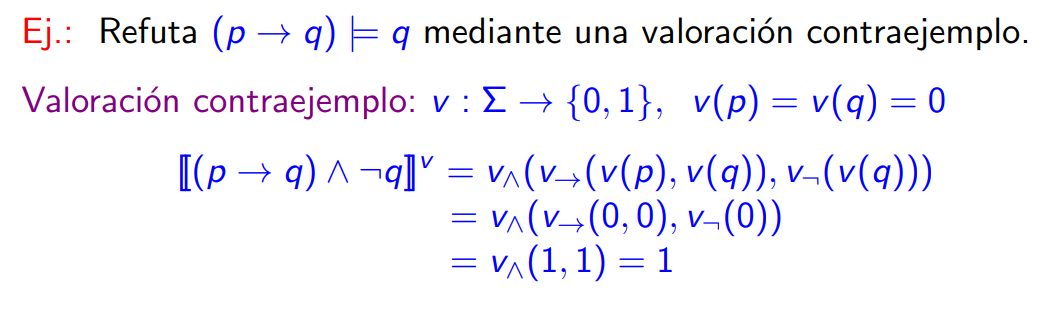
\includegraphics[scale=0.5]{reduccion al absurdo}
\end{center}

\subsection*{\underline{Equivalencia lógica}}
No es difícil ver que si el número de proposiciones en el vocabulario de la fórmula crece, el crecimiento del número de valoraciones es exponencial, más concretamente $2^n$ donde $n$ es el número de proposiciones atómicas. Por ello, es necesario encontrar un método para hallar el valor veritativo de una fórmula o al menos simplificarla para calcularlo sobre una más sencilla.

\subsubsection*{Equivalencia de fórmulas}
Dadas $\varphi, \psi\in L_\Sigma$ decimos que ambas son lógicamente equivalentes cuando el conjunto de modelos de ambas coincide:
$$\varphi \sim \psi \Leftrightarrow Mod(\varphi) = Mod(\psi) \Leftrightarrow \forall v: \Sigma \rightarrow \{0,1\}, \ [\varphi]^v = [\psi]^v$$
La siguiente definición implica que $\varphi \leftrightarrow \psi$ es una tautología y conlleva las siguientes propiedades:
\begin{itemize}
\item La relación $\sim \ \subseteq L_\Sigma \times L_\Sigma$ es una relación de equivalencia.
\item Se tiene que $\varphi\models \psi$ y $\psi \models\varphi$
\item Una fórmula es tautología si y solo si $\varphi \sim \top$
\item Una fórmula es contradicción si y solo si $\varphi \sim \bot$
\item Si tenemos una fórmula $\chi$ en la que aparece $\varphi$, es decir, $\chi(\varphi)$, entonces el sustituir $\varphi$ por $\psi$ en alguna o en todas las apariciones de la misma no influye en la valoración ni significado de la fórmula.
\end{itemize}
Un buen método para poder simplificar por equivalencia lógica estas fórmulas es tener en cuenta las leyes algebraicas de Boole que se pueden aplicar en este caso por formar junto con la función valoración un retículo de Boole:
\begin{center}
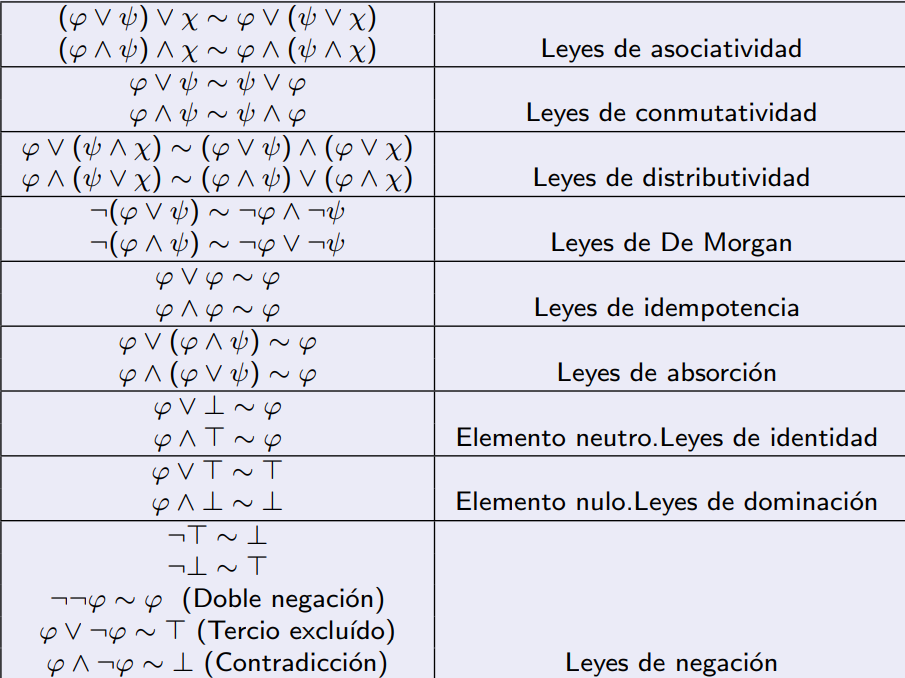
\includegraphics[scale=0.5]{Leyes Algebraicas de Boole}
\end{center}

\subsubsection{Forma normal conjuntiva y disyuntiva}
Relacionado con el concepto anterior de equivalencia lógica, vamos a ver dos formas canónicas a las que se puede convertir cualquier fórmula del lenguaje de la lógica definido. Para ello definimos el concepto de \textbf{literal} como una fórmula del tipo $\varphi$ o $\neg \varphi$, pero no se permiten otras conectivas lógicas entre ellas.
\begin{itemize}
\item \underline{\textbf{Forma Normal Disyuntiva (FND)}}

Se trata de una forma canónica en la que tenemos una serie de cláusulas conjuntivas, esto es, literales unidos entre ellos por conjunciones, unidas por disyunciones entre ellas, es decir:
$$FND\rightarrow (\varphi_1 \wedge \varphi_2 \wedge \cdots \wedge \varphi_n) \vee (\psi_1 \wedge \cdots \wedge \psi_m) \vee \cdots \vee (\chi_1 \wedge \cdots \wedge \chi_s)$$

\item \underline{\textbf{Forma Normal Conjuntiva (FNC)}}

Se trata de una forma canónica en la que tenemos una serie de cláusulas disyuntivas, esto es, literales unidos entre ellos por disyunciones, unidas por conjunciones entre ellas, es decir:
$$FNC\rightarrow (\varphi_1 \vee \varphi_2 \vee \cdots \vee \varphi_n) \wedge (\psi_1 \vee \cdots \vee \psi_m) \wedge \cdots \wedge (\chi_1 \vee \cdots \vee \chi_s)$$
\end{itemize}

Teniendo en cuenta estos dos conceptos podemos asegurar la siguiente afirmación:
$$\forall \varphi \in L_\Sigma: \exists \psi (FND), \chi(FND): \varphi \sim \psi \sim \chi$$
Puesto que si tenemos una fórmula $\varphi$ sabemos que posee unas ciertas valoraciones que son modelos (o ninguna y en ese caso sería $\sim \bot$), de este modo la fórmula es cierta si y solo si son ciertas las condiciones de valoración de los literales de alguno de sus modelos, luego:
$$[\varphi]^v = 1\Leftrightarrow [v_1 \vee v_2 \vee \cdots \vee v_n]^v = 1\Rightarrow \exists \chi (FND)\in L_\Sigma : \psi \sim \varphi$$
Es decir, que pensando en la tabla de verdad de la fórmula, para cada línea que haga 1 la fórmula hay una combinación de 0 y 1 de los literales que identifican dicha línea, por tanto, esos literales van con una conjunción entre ellos y negados o no negados en función de si deben valer 0 o 1 y además todos los modelos van unidos entre ellos por disyunciones puesto que solo es necesario que al menos alguno de ellos sea cierto para que la fórmula sea cierta.

Para ahora obtener la FNC, hallamos la FND de la negación de la fórmula. Como esta FND y $\neg \varphi$ son equivalentes, si la negamos obtenemos de nuevo $\varphi$ por las leyes algebraicas de Boole, pero la negación de una serie de cláusulas conjuntivas unidas por disyunciones es de nuevo por Boole una serie de cláusulas disyuntivas unidas por conjunciones, que además es equivalente a $\varphi$; luego tenemos ya nuestra FNC.

\begin{center}
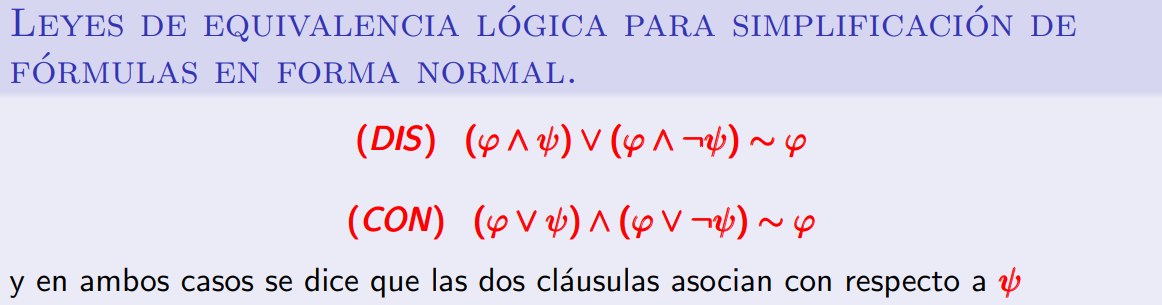
\includegraphics[scale=0.5]{simplificar FND}
\end{center}

\subsection*{\underline{Tableaux semánticos}}
Este método consiste en un algoritmo muy preciso para poder determinar cuando a partir de unas hipótesis algo es consecuencia lógica o no sin necesidad de hacer a mano todas las tablas de verdad y comparar modelos, decidir si un conjunto de fórmulas es satisfactible, saber si algo es tautología y calcular las formas normales.

\subsubsection*{Demostración de la consecuencia lógica}
Para poder demostrar que de un conjunto $\Phi$ de premisas una fórmula $\varphi$ es consecuencia lógica demostramos que $\Phi\cup\{\neg \varphi\}$ es insatisfactible, es decir, refutamos la idea de que las premisas puedan ser ciertas siendo las condiciones falsas.

El procedimiento general parte de la base de ir simplificando y dividiendo en trozos cada una de las fórmulas que componen el conjunto en base a la siguiente clasificación:
\begin{center}
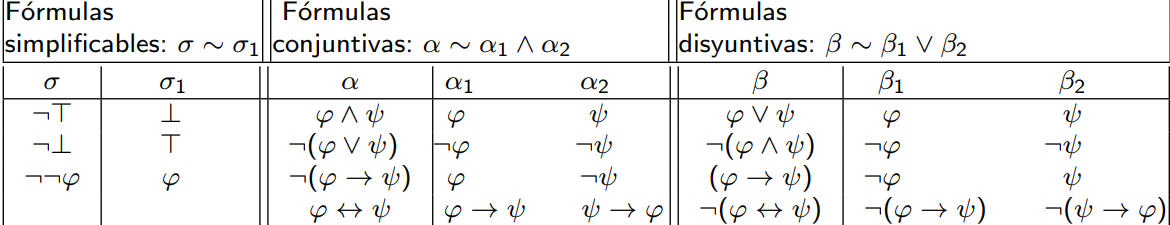
\includegraphics[scale=0.6]{formulas tableaux}
\end{center}

En sí, un tableaux va abriendo los distintos caminos o posibilidades que hacen ciertas a las fórmulas que componen el conjunto. Se trata de construir un árbol (grafo) a partir del tronco formado por las fórmulas iniciales e irlo prolongando en ramas según los escenarios que vayan surgiendo, para ello se siguen las siguientes reglas de formación:
\begin{itemize}
\item $[R_{ini}]$: Para poder comenzar, formamos el tronco del árbol con las fórmulas correspondientes al conjunto y esta será nuestra primera rama.

\item $[R_\sigma]$: Si $\theta$ es una rama abierta de $T$ con un nodo etiquetado con una fórmula simplificable $\sigma$, se obtiene $T'$ \textbf{alargando} la rama $\theta$ con su simplificación $\sigma_1$.

\item $[R_\alpha]$: Si $\theta$  es una rama abierta de $T$ con un nodo etiquetado con una fórmula conjuntiva $\alpha$, se obtiene $T'$ \textbf{alargando} la rama $\theta$ con dos nodos nuevos etiquetados con las componentes de la conjunción $\alpha_1$ y $\alpha_2$.

\item $[R_\beta]$: Si $\theta$ es una rama abierta de $T$ con un nodo etiquetado con una fórmula disyuntiva $\beta$, se obtiene $T'$ \textbf{dividiendo} a la rama $\theta$ en otras dos y usando como hijos las componentes $\beta_1$ y $\beta_2$.
\end{itemize}
Nuestro objetivo es aplicar de forma sucesiva todas estas reglas hasta llegar a un tableaux equivalente simplificado que no pueda reducirse más, en ese caso decimos que el tableaux queda terminado. 

Cuando en uno de los caminos (recorridos desde el tronco hasta el final de una rama, \textbf{pero no entre ramas}) encontramos una fórmula $\varphi$ y su negada $\neg \varphi$, entonces decimos que esa rama está cerrada, puesto que hemos llegado a un escenario imposible. \textbf{En consecuencia, si algo es consecuencia lógica de un conjunto de premisas, entonces al incorporarlo negado al mismo el tableaux correspondiente será cerrado en todas sus ramas}.

\subsubsection*{Satisfacibilidad de un conjunto de fórmulas}
En el proceso de demostración de una deducción lógica hemos refutado que $\Phi\cup\{\neg\varphi\}$ sea satisfactible, por lo que ya sabemos como probar la satisfacibilidad de un conjunto de fórmulas; basta con ver que el tableaux que podemos construir con ellas es cerrado en todas sus ramas.

Si un tableaux que ha sido terminado todavía posee ramas abiertas, podemos asociar ese caso particular la valoración que hace que el conjunto no sea insatisfactible, dicha valoración quedará definida de la siguiente forma:
$$v_\theta = \{v_\theta (p_1), \cdots, v_\theta (p_n)\}: v_\theta (p_i) = \begin{cases} 1 & \mbox{ si p aparece en }\theta \\ 0 & \mbox{ si }\neg p\mbox{ aparece en }\theta \\ \mbox{ arbitrario} & \mbox{ si no aparece en }\theta \end{cases}$$
Para el caso de la deducción lógica, esta valoración $v_\theta$ es una valoración contraejemplo.

\subsubsection*{Cálculo de formas normales}
Dada una fórmula $\varphi \in L_\Sigma$	podemos determinar su FND construyendo el tableaux asociado a dicha fórmula y podemos encontrarnos dos escenarios:
\begin{itemize}
\item Tableaux cerrado: en cuyo caso $FND(\varphi) = \bot$
\item Tableaux abierto: en cuyo caso se construye una conjunción de todos los literales que aparezcan en la rama, es decir, que se escribe cada término $p_i$ de la valoración $v_\theta$ con el símbolo $\neg$ delante o no en función de si la valoración particular de ese término es 1 o 0.
\end{itemize}
Para obtener la FNC se realizan las conversiones pertinentes explicadas en su capítulo.




\chapter*{LÓGICA DE PREDICADOS}
Es claro que para la lógica desarrollada hasta ahora, a pesar de ser correcta, se tienen ciertas insuficiencias que no permiten desarrollar razonamientos más complejos con le lenguaje definido. Por ejemplo, nuestros razonamiento con frecuencia aluden a individuos como elementos de un colectivo y no como individuos y eso hace que enunciados como (poner ejemplo) no sean capaces de ser procesados por la lógica proposicional.

Para poder extender la lógica proposicional a un ámbito mucho más general y que permita desarrollar razonamientos más complejos necesitamos hacer una \textbf{extensión} de la misma, es decir, vamos a agregar los siguientes elementos:
\begin{itemize}
\item \textbf{Dominio o universo del discurso}: denota el colectivo de individuos sobre el que razonamos.
\item \textbf{Constantes}: denotan los nombres propios que hacen referencia a individuos concretos del conjunto.
\item \textbf{Variables}: denotan los valores cualesquiera del universo y permiten referirse a un individuo cualquiera de forma anónima.
\item \textbf{Predicados}: son los enunciados sobre los individuos y hay de dos tipos:
	\begin{itemize}
	\item Monádicos: que hacen referencia a propiedades de un individuo y le atribuye alguna propiedad.
	\item Poliádicos: que hacen referencia a propiedades de las relaciones entre individuos.
	\end{itemize}

\item \textbf{Funciones}: son enunciados que describen un individuo en función de otro.

\item \textbf{Símbolo de igualdad}: expresa la relación de igualdad entre dos términos.

\item \textbf{Cuantificadores}: redefinen los predicados indicando la frecuencia con la que ocurre una afirmación.
	\begin{itemize}
	\item Cuantificador universal: indica que algo es cierto para todos los individuos del colectivo.
	\item Cuantificador existencial: indica que algo es cierto para al menos alguno de los individuos del colectivo.
	\end{itemize}
\end{itemize}
En definitiva, este nuevo concepto de lógica permite profundizar mucho más allá en los razonamientos vistos y no prescinde de la lógica anterior, sino que la incorpora y la mejora.

\section*{DEFINICIÓN Y LENGUAJE DE LA LÓGICA}
\subsection*{\underline{Sintaxis de la lógica de 1º orden}}
\subsubsection*{Alfabeto de símbolos primitivos}
De nuevo, para poder definir cualquier lenguaje, en este caso el de la lógica de primer orden, necesitamos definir un alfabeto sobre el cual no haya interpretaciones posibles sobre el significado que le queremos atribuir a un enunciado concreto. Para ello, vamos a incorporar al alfabeto que teníamos en la lógica proposicional una serie de cambios y además redefinir en parte algunos conceptos:
\begin{itemize}
\item \underline{\textbf{Símbolos lógicos}}: $\{\bot, \top, \neg, \wedge, \vee, \rightarrow, \leftrightarrow, \forall, \exists, =\}$
	\begin{itemize}
	\item \textbf{Conectivas proposicionales}: $\{\bot, \top, \neg, \wedge, \vee, \rightarrow, \leftrightarrow\}$.
	\item \textbf{Cuantificadores}: $\{\forall, \exists\}$ denotando universal y existencial respectivamente.
	\item \textbf{Signo de igualdad}: $\{=\}$ denotando igualdad entre términos.
	\end{itemize}
\item \underline{\textbf{Símbolos auxiliares}}: $\{(, ), \ ,\}$

Son símbolos que denotan la precedencia de operadores o el radio de alcance de los cuantificadores.

\item \underline{\textbf{Conjunto de Variables}}: $V=\{x,y,z,w,t, \cdots\}$

Es un conjunto infinito numerable de símbolos que denotan variables.

\item \underline{\textbf{Signatura}}: $\Sigma$

Denotamos por $\Sigma$ al conjunto de símbolos de función y predicado con sus respectivas aridades\footnote{Número de argumentos} asociadas, por tanto, podemos considerar:
$$\Sigma = F_\Sigma \cup P_\Sigma: \begin{cases} F_\Sigma = \{f \mbox{ función }\} \\ P_\Sigma = \{P \mbox{ predicado}\}\end{cases}$$
Además, si queremos especificar la aridad asociada a cada conjunto denotamos:
\begin{align*}
F_\Sigma^n & = \{f\in F_\Sigma: ar(f)=n\} & P_\Sigma^n & = \{P\in P_\Sigma: ar(P)=n\}
\end{align*}
Por último, consideramos a las funciones de aridad 0 como \textbf{constantes} y las denotaremos por letras minúsculas $a,b,c,d, \cdots$ y consideraremos los predicados de aridad 0 como \textbf{proposiciones} denotándolas por letras minúsculas $p,q,r,\cdots$
\end{itemize}
Por tanto, tras describir todos los símbolos que van a ser empleados y dotarlos de una función inequívoca, nos queda el siguiente alfabeto:
$$A_\Sigma = \Sigma \cup \{(,), \ ,\}\cup \{\bot, \top, \neg, \wedge, \vee, \rightarrow, \leftrightarrow, \forall, \exists, =\}\cup V$$

\subsubsection*{Lenguaje de la lógica de 1º orden}
Una vez construido el alfabeto sobre el que se basará nuestro lenguaje, es necesario establecer unas normas para determinar qué palabras sobre ese alfabeto son válidas o no. En primer lugar, en este tipo de lógica se pueden construir 2 expresiones:
\begin{itemize}
\item \underline{\textbf{Términos}} ($T_\Sigma$): designan individuos del universo del discurso.
\item \underline{\textbf{Fórmulas}} ($L_\Sigma$): representan enunciados sobre términos concretos.
\end{itemize}
Con cual para poder construir las distintas expresiones hay que ceñirse al siguiente conjunto de normas:

\underline{\textbf{Reglas de formación de términos}}:

Denotamos al conjunto de términos sobre la signatura $\Sigma$ como $T_\Sigma$ y el conjunto lo forman las palabras construidas sobre el alfabeto $A_\Sigma$ conforme al siguiente conjunto de normas:
\begin{itemize}
\item Las variables son términos atómicos
\item Las constantes son términos atómicos
\item Si tenemos $t_1, \cdots, t_n \in T_\Sigma$ y $f\in F^n_\Sigma$, entonces $f(t_1, \cdots, t_n)$ es un término
\end{itemize}

\underline{\textbf{Reglas de formación de fórmulas}}:

Denotamos al conjunto de fórmulas sobre la signatura $\Sigma$ como $L_\Sigma$ y el conjunto lo forman las palabras construidas sobre el alfabeto $A_\Sigma$ conforme al siguiente conjunto de normas:
\begin{itemize}
\item Las construcciones que hemos calificado como proposiciones son fórmulas atómicas.
\item Si $s,t\in T_\Sigma$, es decir, son términos, entonces $s=t$ es una fórmula atómica.
\item Si $t_1, \cdots, t_n\in T_\Sigma$ y $P\in P_\Sigma^n$, entonces $P(t_1,\cdots, t_n)$ es una fórmula atómica.
\item Si $\varphi \in L_\Sigma$, entonces $\neg \varphi$ es una fórmula compuesta.
\item Si $\varphi_1, \varphi_2\in L_\Sigma$, entonces $\varphi_1 \square \varphi_2$ es una fórmula compuesta (siendo $\square$ alguna conectiva lógica binaria).
\item Si $\varphi\in L_\Sigma$ y $x\in V$, entonces $\forall x, \ \varphi$ es una fórmula compuesta llamada cuantificación universal.
\item Si $\varphi\in L_\Sigma$ y $x\in V$, entonces $\exists x, \ \varphi$ es una fórmula compuesta llamada cuantificación existencial.
\end{itemize}

\end{document}
